\documentclass[12pt]{article}
\usepackage[utf8]{inputenc}
\usepackage{amsmath}
\usepackage{amsfonts}
\usepackage{amssymb}

\usepackage[margin=1in]{geometry} %1inch margins
\usepackage{graphicx} %for picture inclusion
\graphicspath{ {Figures/} }
\usepackage[backend=bibtex]{biblatex} %for references
\addbibresource{ref.bib} % bibliography info file
\usepackage{authblk} %for titles
\usepackage{verbatim}

\begin{document}

\author{Daniel Gawerc\\Mentor: Maria Spiropulu\\Co-Mentor: Cristian Peña}
\affil{California Institute of Technology}
\title{Progress Report \#2}
\date{29 July 2016}
\maketitle

\section{Background}
At the Large Hadron Collider (LHC), the High Luminosity upgrades plan to achieve luminosities of greater than $10^{34}$ cm$^{-2}$s$^{-1}$, with 140 – 200 pileup events per bunch crossing every 25 ns \cite{P1}. 
Because of the physical spread of each bunch, the collisions occur over a large region rather than at an isolated point, which leads to a spread in time ($\sim$ 200 ps) \cite{P1}. 
Thus, detectors in the calorimeter must have a good (low) time resolution in order to resolve individual collisions. 
In order to reconstruct the vertex of a collision with an increased pileup, the electromagnetic calorimeter (ECAL) detectors should have a time resolution of about 10 ps \cite{P1}.


\section{Experimental Setup}
This summer, the Caltech Precision Timing group took data at the Fermilab Test Beam Facility (FBTF). 
The experiment involves placing different calorimeter detectors in the beam line, in order to observe how the addition of detectors in the perpendicular transverse plane and/or parallel longitudinal direction along the beam line will improve the overall detector time resolution. 
The layers of detectors are meant to mimic the proposed High Granularity Calorimeter (HGC) detector, which shall replace the CMS ECAL endcap, and is described in detail below \cite{P2}. 
The results of this research may be useful in preparing the LHC High Luminosity upgrades.

In the FTBF experiment, different types of detectors were utilized. 
In the front of the setup, a scintillator crystal and PMT are used as a trigger. 
Depending on the configuration, there are a few radiation lengths ($X_0$) of either lead or tungsten absorbers behind the PMT in order to spread out and propagate the particle shower and produce more secondary electrons and photons. 
A depiction of the setup is given in Figure \ref{fig:setup}.

\begin{figure}[h]
	\centering
	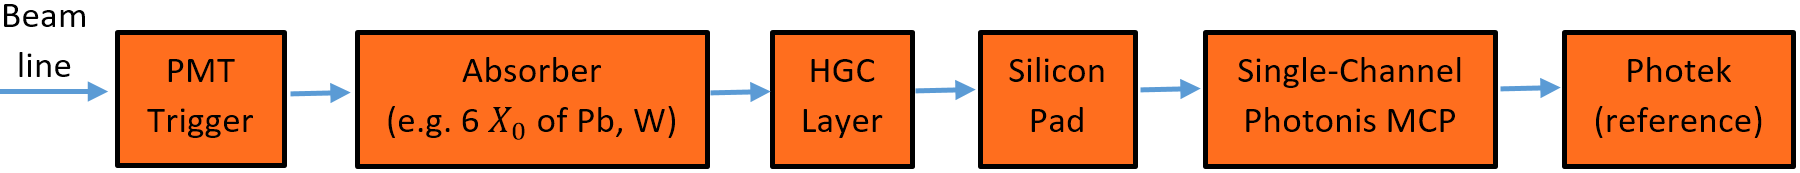
\includegraphics[width=\linewidth]{setup.png}
	\caption{A typical experiment configuration.}
	\label{fig:setup}
\end{figure}

\begin{figure}[h]
\centering
\begin{minipage}[t]{.5\textwidth}
	\centering
	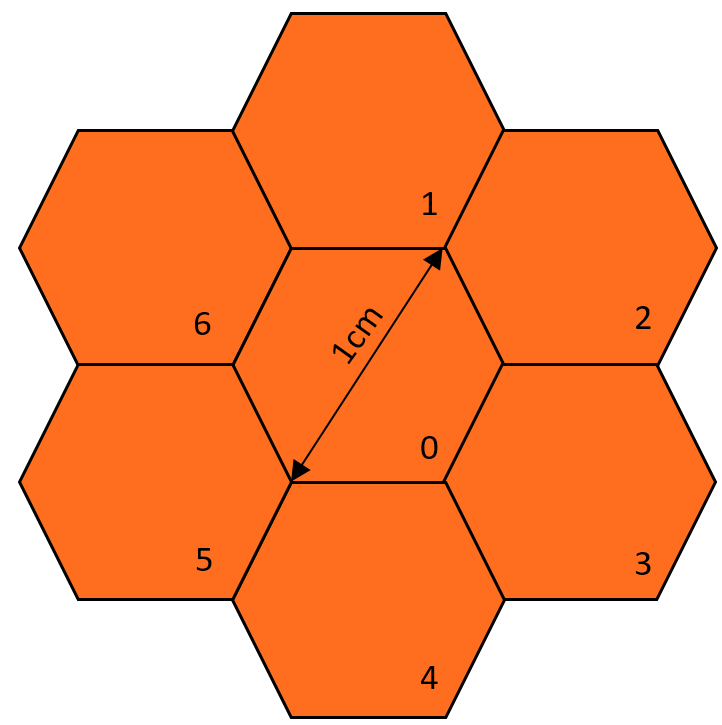
\includegraphics[scale=0.5]{HGC.png}
	\caption{A depiction of the innermost 7 pixels of the HGC layer. 
	The actual board has more than 7 pixels in a single layer.}
	\label{fig:HGC}
\end{minipage}
\end{figure}

The High Granularity Calorimeter (or PicoSil when referring to a single pixel’s readout that has been optimized for timing) layer has an array of separated silicon pixels, in a hexagonal honeycomb geometry \cite{P2}. 
A depiction of the HGC layer is given in Figure \ref{fig:HGC}. 
Because the beam is focused at the HGC center pixel (0 in Figure \ref{fig:HGC}), its signal is reduced using a 6 dB attenuator due to the high charge detected relative to other pixels. 

The Photek 240 MCP is used as a reference detector because its time resolution is good ($\sim$ 10 ps). 
Because the readout board for all the detectors is divided into 4 groups, which have some time delay between them, the Photek signal is split into 4 cables and plugged into each group as the reference signal from which the TOFs (time of flight, or $\Delta t$) are calculated. 
Specifically, the time taken for the particle to travel from a device to the reference Photek - the time of flight – is represented by $\Delta t$. 
In the data analysis, the $\Delta t$ values over all events in the run (with certain \textit{bad} events excluded) are combined in a histogram, forming a Gaussian peak. 
The peak $\sigma$ parameter is denoted the time resolution.

There is a 64-channel and a single-channel Photonis MCP. 
The 64-channel Photonis was not present for most runs, and the single-channel Photonis was instead used. 
Lastly, a silicon pad (SiPad) detector was present for most runs, however it only detected pulses well in the very early runs, and does not seem to be useful in most of the analysis.

\section{Data Analysis}
This section aims to explain the general data analysis methods discussed later in this report.

\subsection{Data Analysis: Overview}
The Caltech Precision Timing group already had developed some analysis code for previous test beam experiments. 
The program \textit{dat2rootCP} analyzes the .dat files (with low-level information) from the runs and turn them into .root files containing a tree with plots and fit results (higher-level information). 
Since some of the data contained ringing noise, which often resulted in the wrong peak being identified as the pulse, \textit{dat2rootCP} was updated to correct for these events. 
Additionally, new macros were written in order to automate batch file analyses and merging the results into a single .root file (for when the setup configuration and beam type were the same over many runs). 
These programs utilize the ROOT programming language, which is based largely on C++. 
It is the main programming language used by scientists at CERN and in the field of HEP (see: root.cern.ch).  
The .root file extensions are associated with the ROOT language.

Because the HGC layer has multiple pixels, each pixel detects different signals and has a different time resolution. 
The \textit{MultiChannelStudy} code was created (here channel and pixel are used interchangeably), which calculates and combines the TOF ($\Delta t$) histograms for different pixels in order to return a better overall time resolution. 
The $\Delta t$ values are calculated for every event in a run by subtracting the pulse time in one device from the pulse time in the Photek (making sure that it is from the same cabling group 1-4 as the device). 
A 1-D histogram is then filled event-by-event with the $\Delta t$ values. 
In an ideal world with perfect detectors and no variation in each event, the histogram would be a Dirac delta function with a time resolution of zero. 
However, due to detector jitter, the signal-to-noise ratio and the particle shower development in the material will vary event-by-event, resulting in Gaussian TOF histograms \cite{P2}. 
After fitting the histogram to a Gaussian, the $\sigma$ parameter gives the time resolution of the detector/pixel. 
If weighted correctly, combining the HGC pixels’ $\Delta t$ histograms will result in a combined histogram with better time resolution (smaller $\sigma$). 
This improvement is due to the combination of non-overlapping information about the shower size and development in each of the detectors.

Because there are also multiple devices along the beam line as well as multiple HGC pixels, the analysis of the coplanar HGC pixels has been called \textit{transverse analysis}, and the analysis of multiple devices \textit{longitudinal analysis}. 
This report shall deal mainly with the longitudinal analysis: analyzing the improvement in the time resolution when taking the HGC layer, single-channel Photonis MCP, and SiPad into account. 
However since it is best to use the time resolution from the entire HGC layer, much of the transverse analysis will be included as well. 
Due to re-cabling the wires of the detectors into different groups between runs 52 and 53, multiple longitudinal analysis codes were written for each setup. 
Additionally, the silicon pad has noise dominating for most of the runs, and substantially deteriorates the combined detector time resolution. 
For example, Figures \ref{fig:Center} and \ref{fig:MCP} give the time of flight ($\Delta t$) histograms for runs 65-83 (same configuration) for the HGC center pixel and the Photonis MCP, along with their Gaussian fit $\sigma$ parameter. 
The Gaussian fit used the log-likelihood maximization method, as the $\chi^2$ minimization method is incorrectly biased by histogram bins with few/empty events.
Figure \ref{fig:SiPad} gives the TOF histogram for the silicon pad. 
Figure \ref{fig:wctc} is one possible combination histogram (more details below on how the individual device $\Delta t$'s can be combined). 
Clearly the combined histogram improves the silicon pad resolution by about 4 times, but it is 4-5 times \textit{worse} than the individual resolutions of the HGC and MCP. 
Additionally, the silicon pad histogram is peaked, but certainly not Gaussian. 
Thus, because it is usually more favorable (in most - but not all - runs) to simply exclude the silicon pad, code that does not account for the silicon pad was also created.

Therefore, because of the change in cabling and the noise in the silicon pad, the following longitudinal analysis codes were used: \textit{MultiDeviceStudy}, \textit{MultiDeviceStudy\_InitialWiring}, \textit{MultiDeviceStudy\_PicosilMCP}, and \textit{MultiDeviceStudy\_InitialWiring\_PicosilMCP}. 
Because the most applicable file is \textit{MultiDeviceStudy\_PicosilMCP}, it is more extensive than the others, incorporating all of the ring 1 pixels (the 6 pixels surrounding the center pixel; refer to Figure \ref{fig:HGC}) in the analysis. 
Thus, the code implements transverse analysis of the HGC as well as longitudinal analysis by adding the Photonis MCP.

\begin{figure}[h]
\centering
\begin{minipage}[t]{.49\textwidth}
	\centering
	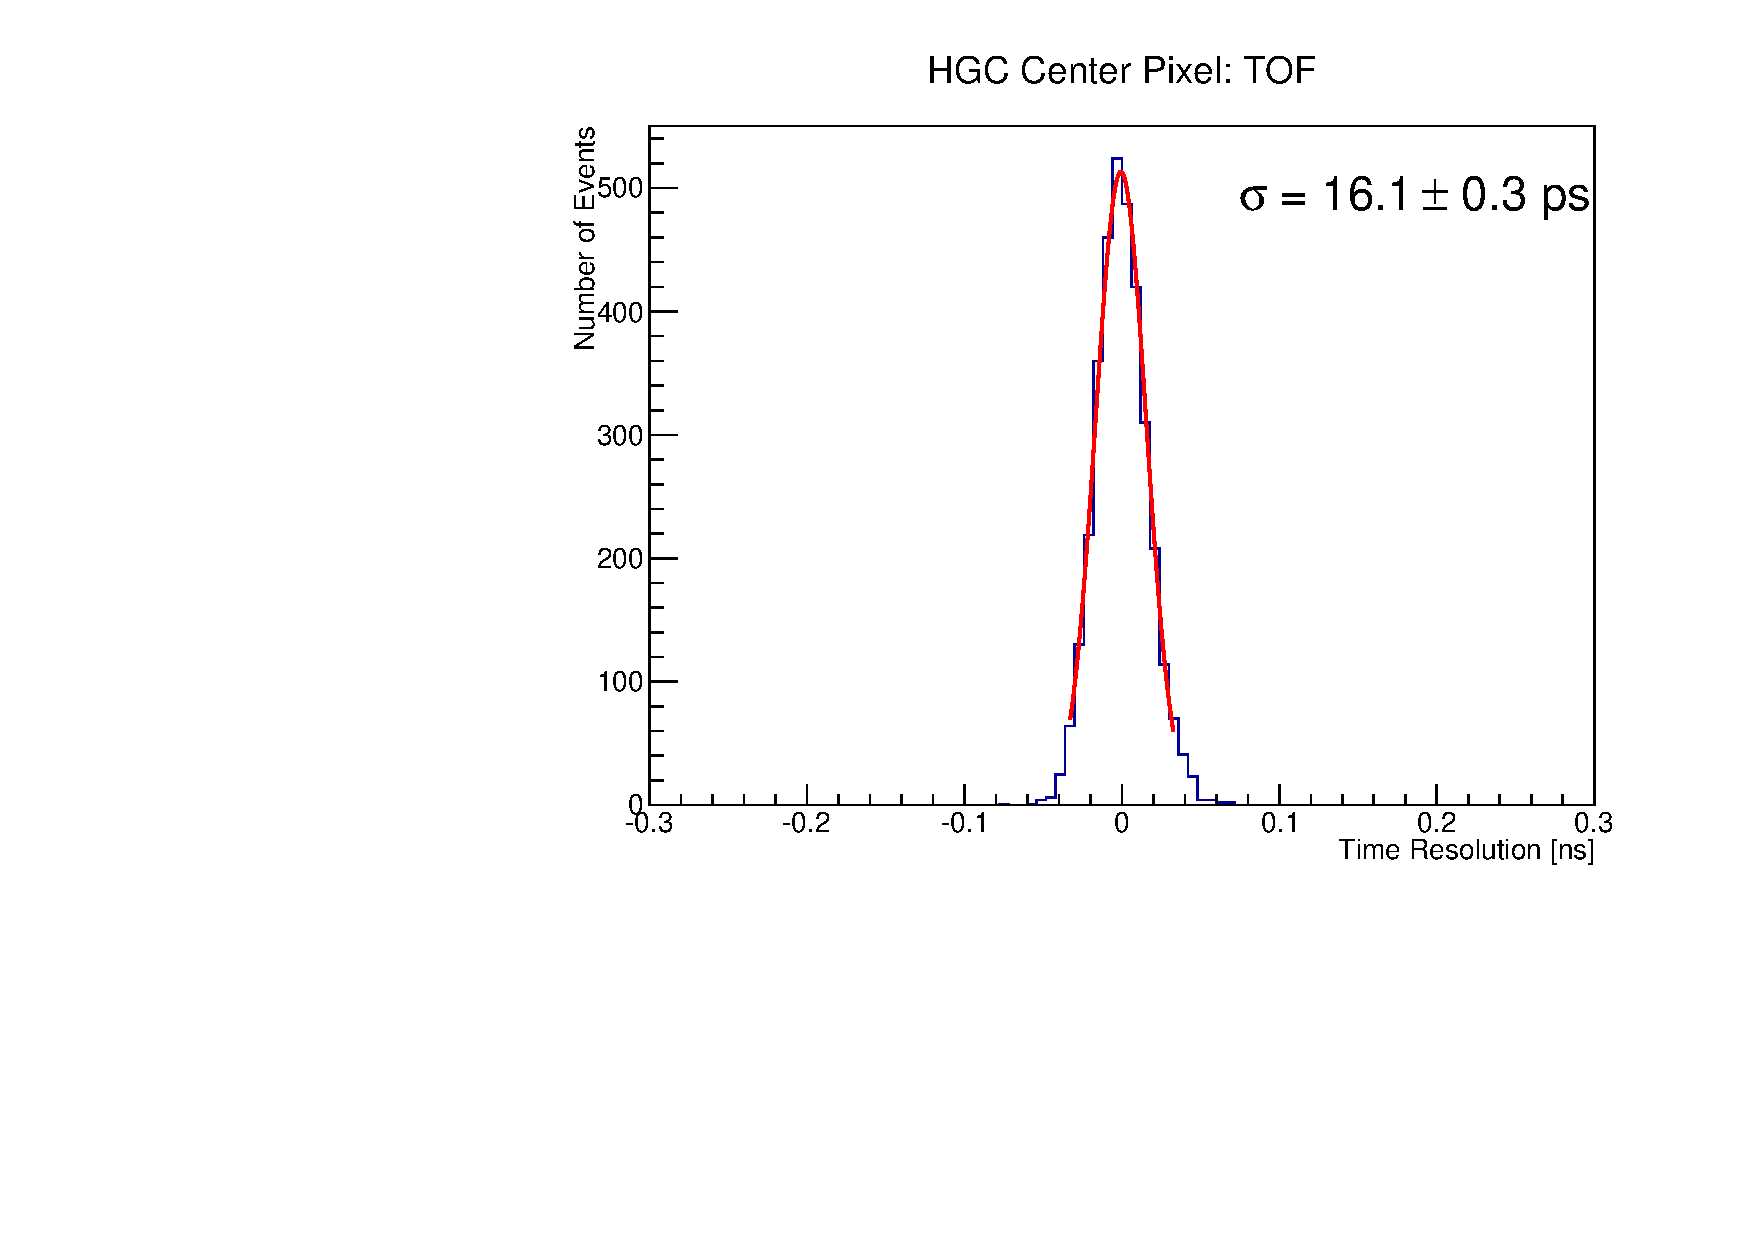
\includegraphics[width=\textwidth]{deltaTCenter.pdf}
	\caption{TOF of the HGC Center Pixel}
	\label{fig:Center}
\end{minipage} \hfill
\begin{minipage}[t]{.49\textwidth}
	\centering
	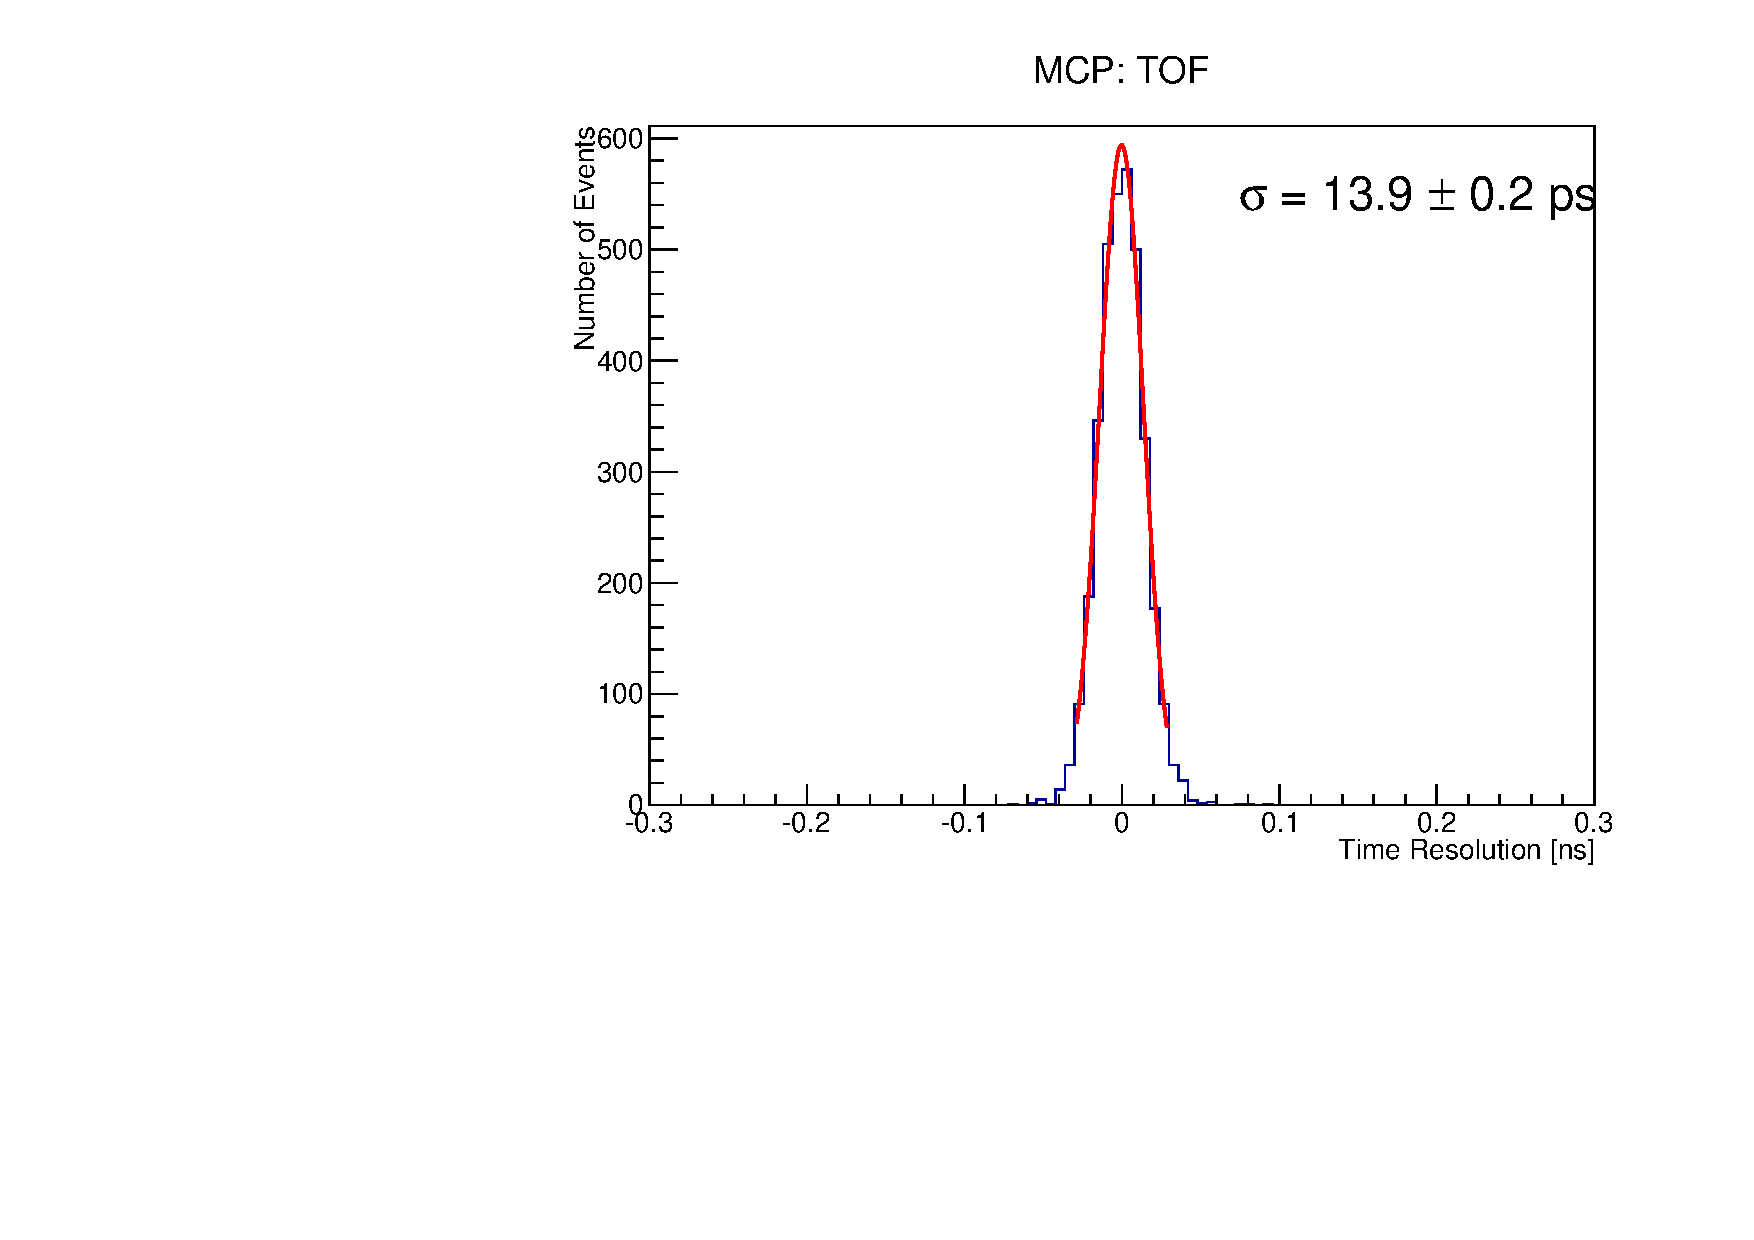
\includegraphics[width=\textwidth]{deltaTMCP.pdf}
	\caption{TOF of the Single-Channel Photonis MCP}
	\label{fig:MCP}
\end{minipage}
\end{figure}

% The following 2 plots are actually a bit out of date, and were combined with slightly
% different versions of the two above plots. Main point is still correct. Would need to
% update the below plots for any final paper.
\begin{figure}[h]
\centering
\begin{minipage}[t]{.49\textwidth}
	\centering
	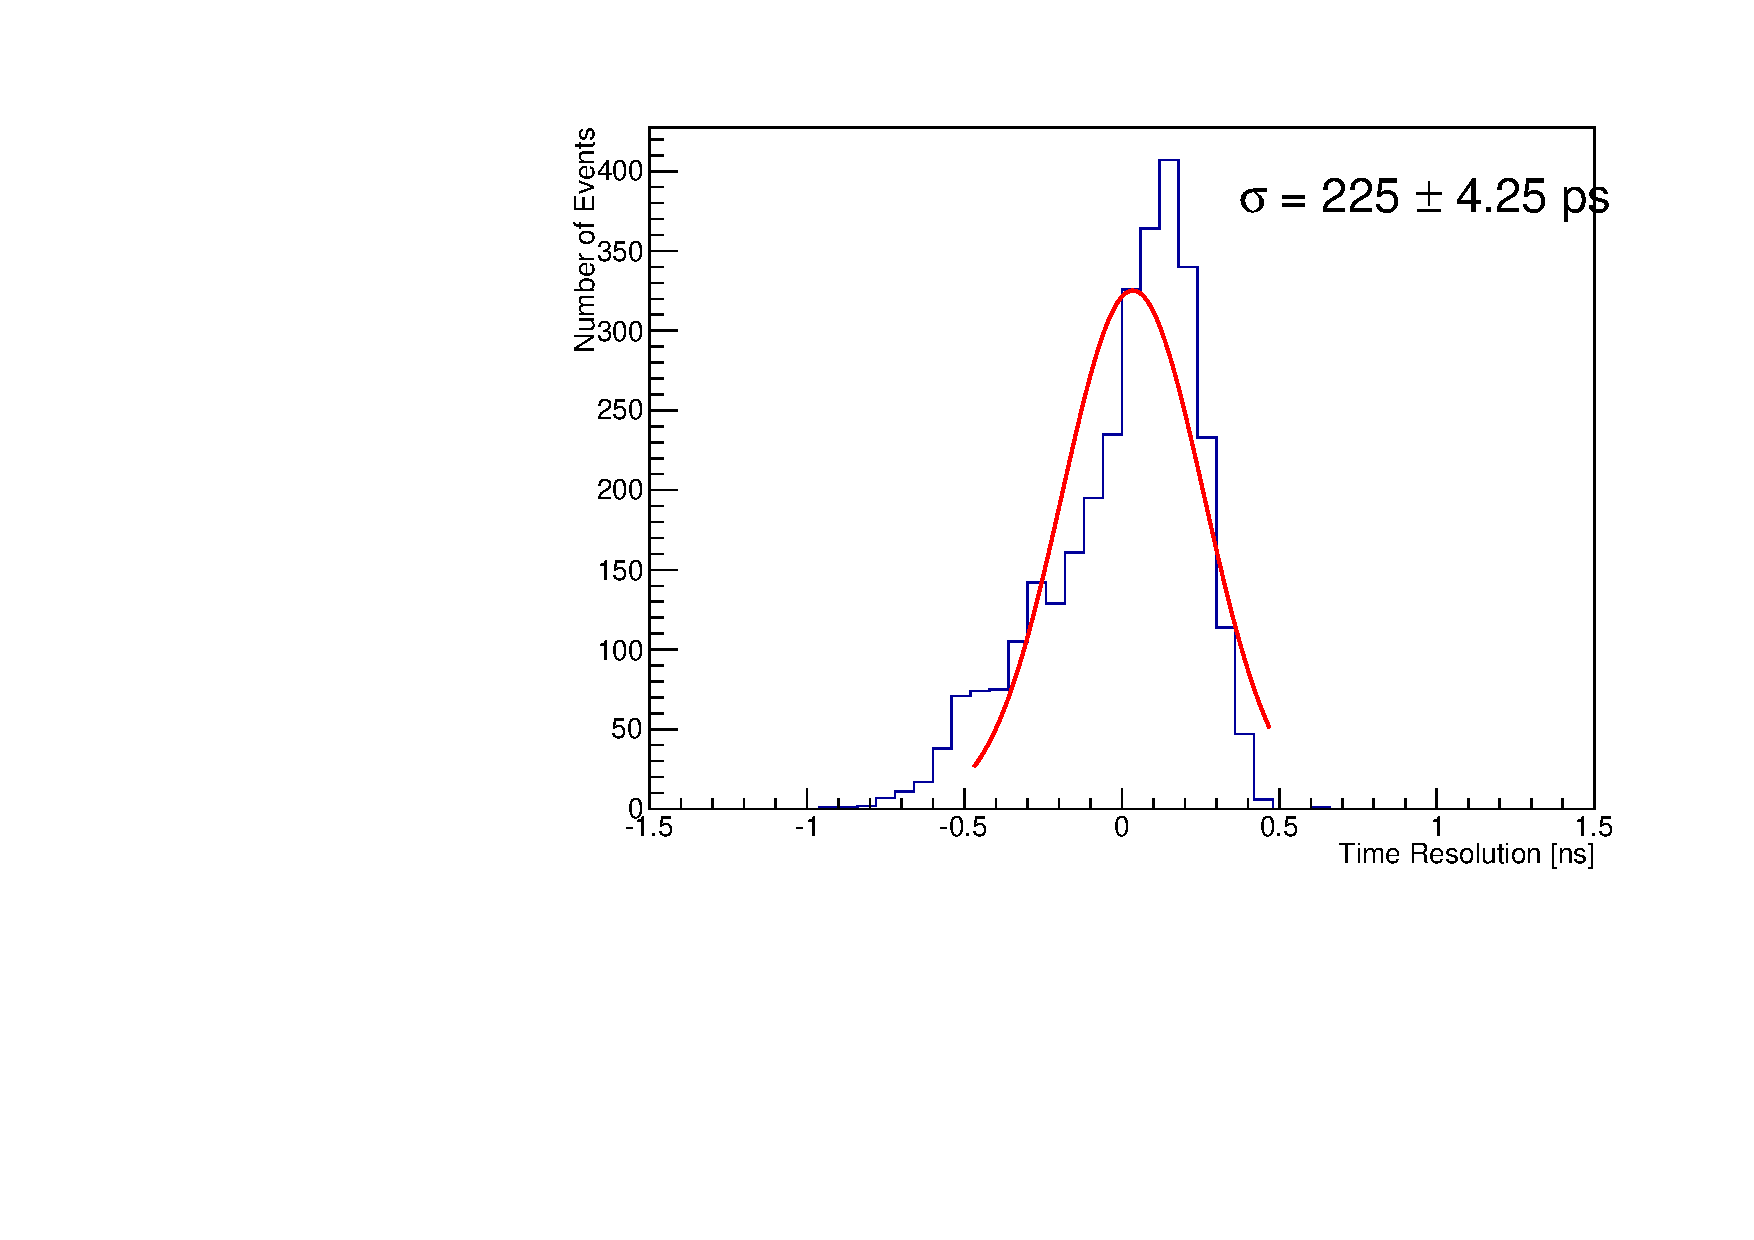
\includegraphics[width=\textwidth]{deltaTSiPad.pdf}
	\caption{TOF of the Silicon Pad}
	\label{fig:SiPad}
\end{minipage} \hfill
\begin{minipage}[t]{.49\textwidth}
	\centering
	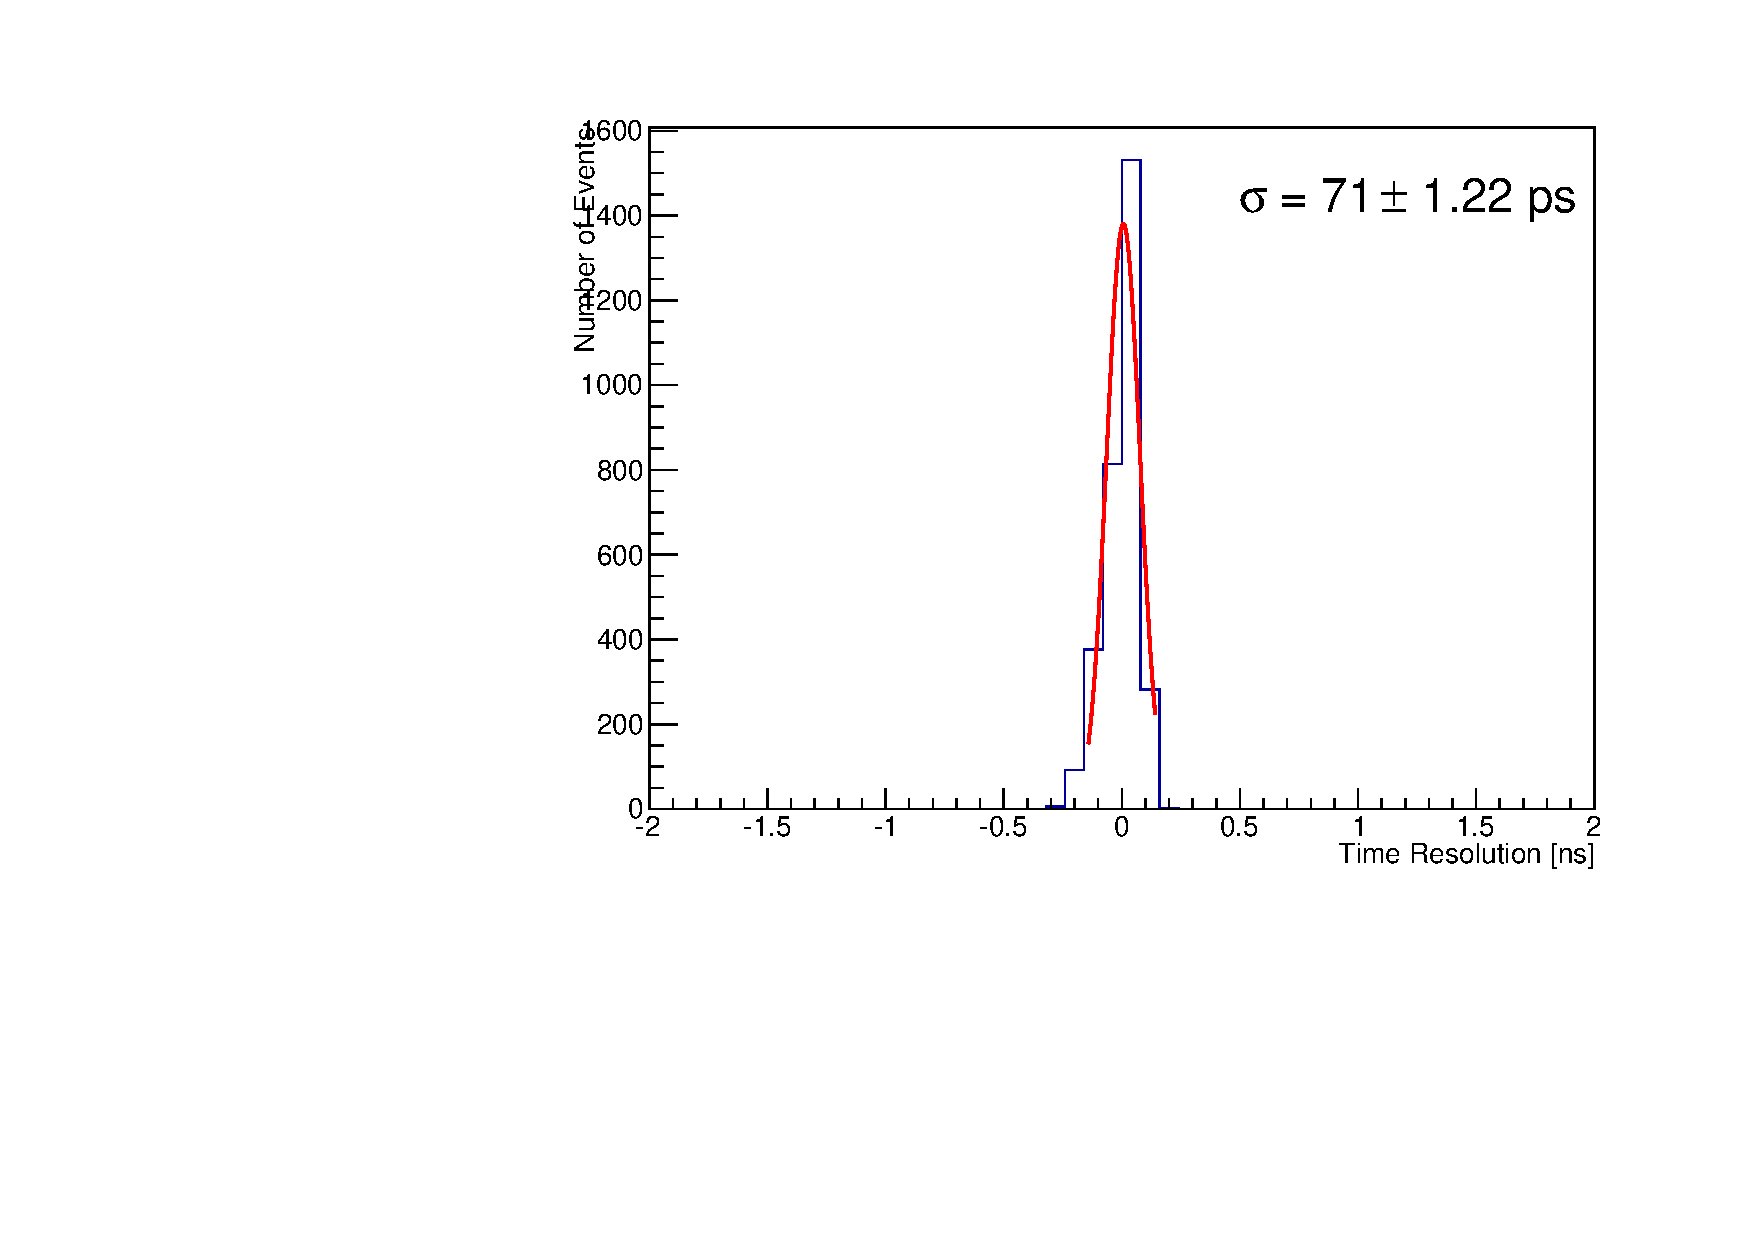
\includegraphics[width=\textwidth]{deltaTWeightsCorrected_totalcharge.pdf}
	\caption{TOF of the HGC Center Pixel, Photonis, and Silicon Pad Combined with Total Device Charge Weighting}
	\label{fig:wctc}
\end{minipage}
\end{figure}


\subsection{Data Analysis: Event Selection}
Before discussing the various ways to combine the $\Delta t$ values from different detectors, the methodology for selecting events that contribute to their individual TOF histograms should be reviewed.
Because not every event contains a detected pulse, and some have a lot of ringing noise and a small signal-to-noise ratio, some events need to be cut out of the $\Delta t$ calculations. 
In order to ensure that most of the \textit{"bad"} events are removed from the histograms, a cut is applied to the calculated peak amplitude (in mA) and to the overall charge (in pC) of the event in that detector, forcing them both to be higher than some threshold. 
This requires that the peak found is not just noise and that the charge (found by integrating the plot) is significant enough to represent a pulse.

For example, analyzing the data (with \textit{dat2rootCP}) from runs 65-83 returns a maximum amplitude value in the Photek for every event. 
Filling a histogram with all of these values in the command-line in ROOT gives the left plot in Figure \ref{fig:AmpCut}. 
Clearly the amplitudes that are near zero or negative are events without pulses or very noisy events. 
These events should be ignored, so a cut is implemented to select for amplitudes above a certain value. 
In this case the value appears to be $0.1\times\sqrt{10}$ mA. 
The right plot in Figure \ref{fig:AmpCut} shows the histogram of the amplitudes with only the events that passed the cut. 
Figure \ref{fig:ChargeCut} shows the same methodology being applied to the charge distribution, with a cut at $2\times\sqrt{10}$ pC. 
Similar cuts were made in the HGC pixels and Photonis MCP. 

\begin{figure}[h]
\centering
	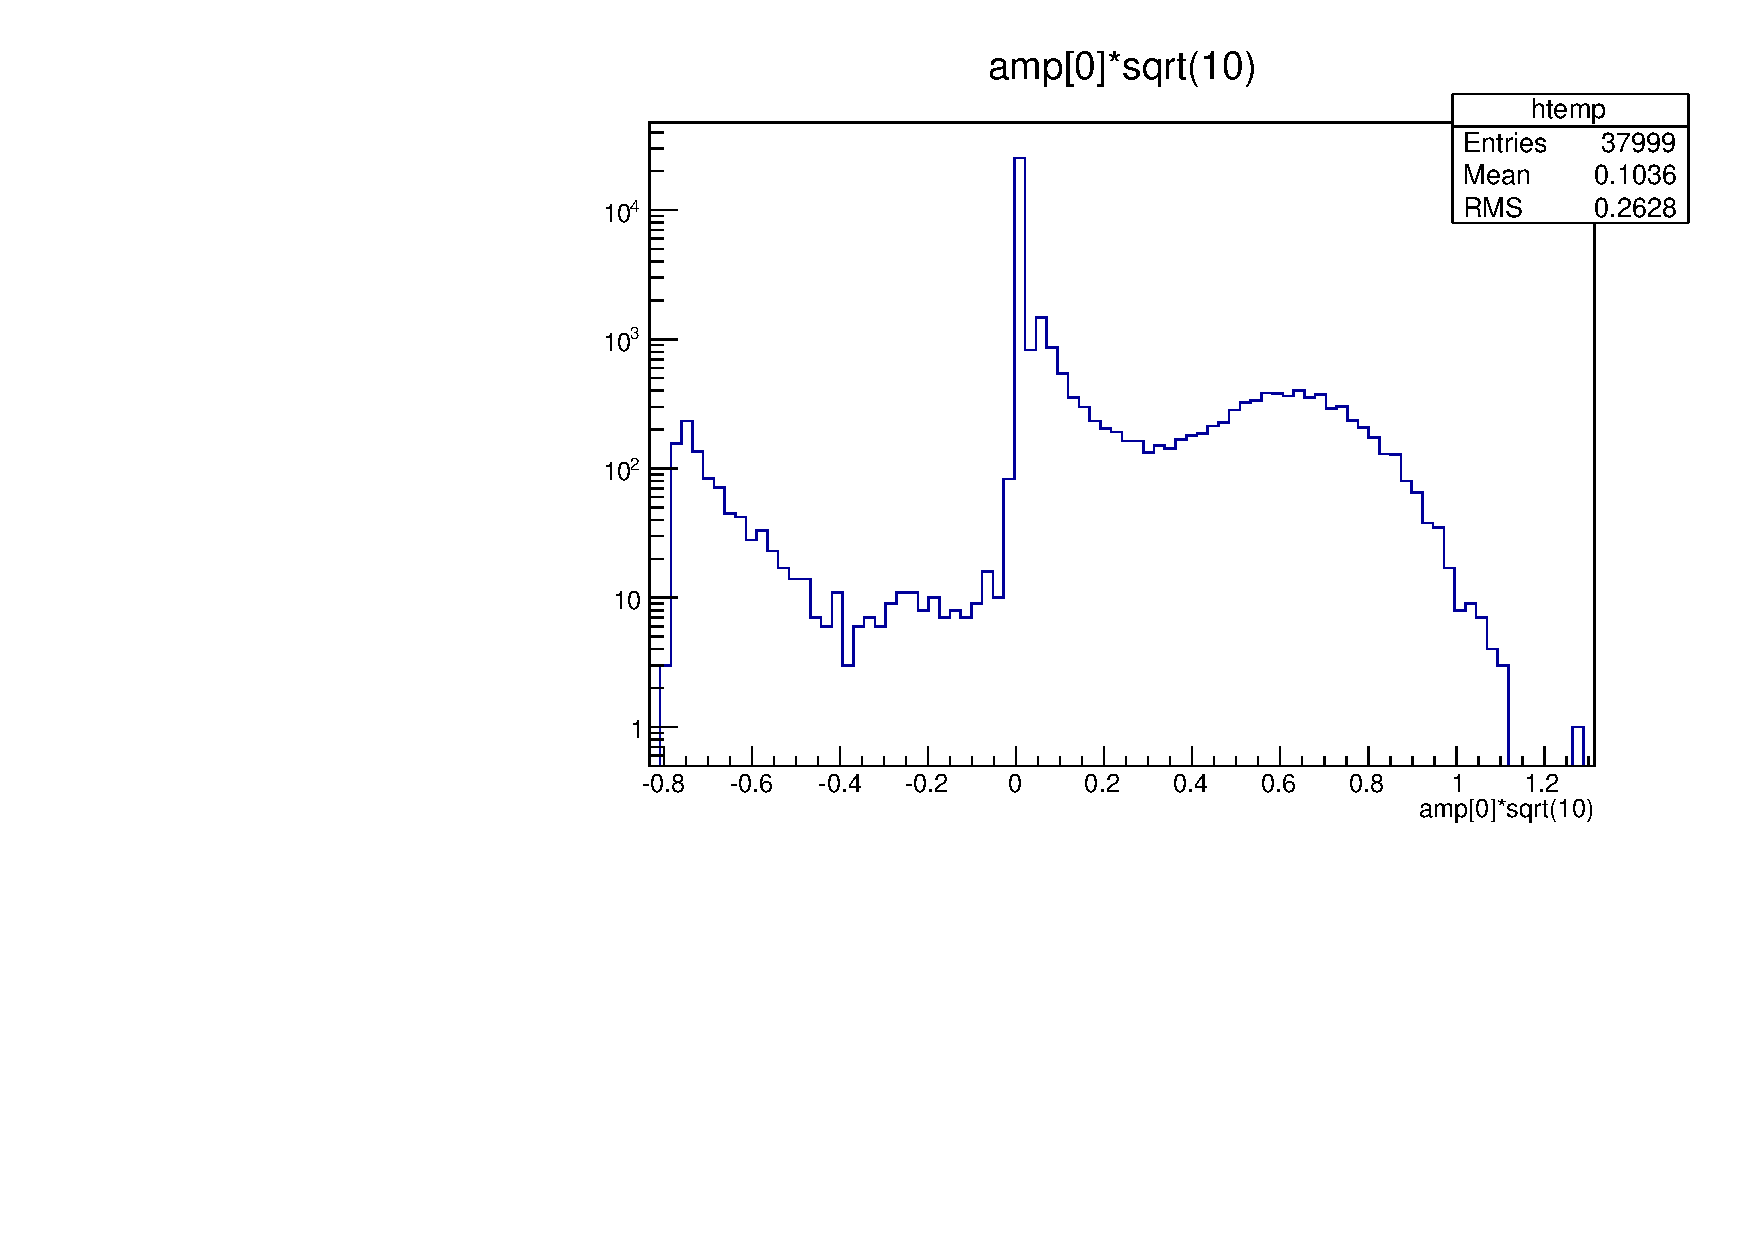
\includegraphics[width=0.49\textwidth]{AmpCut0.pdf}
	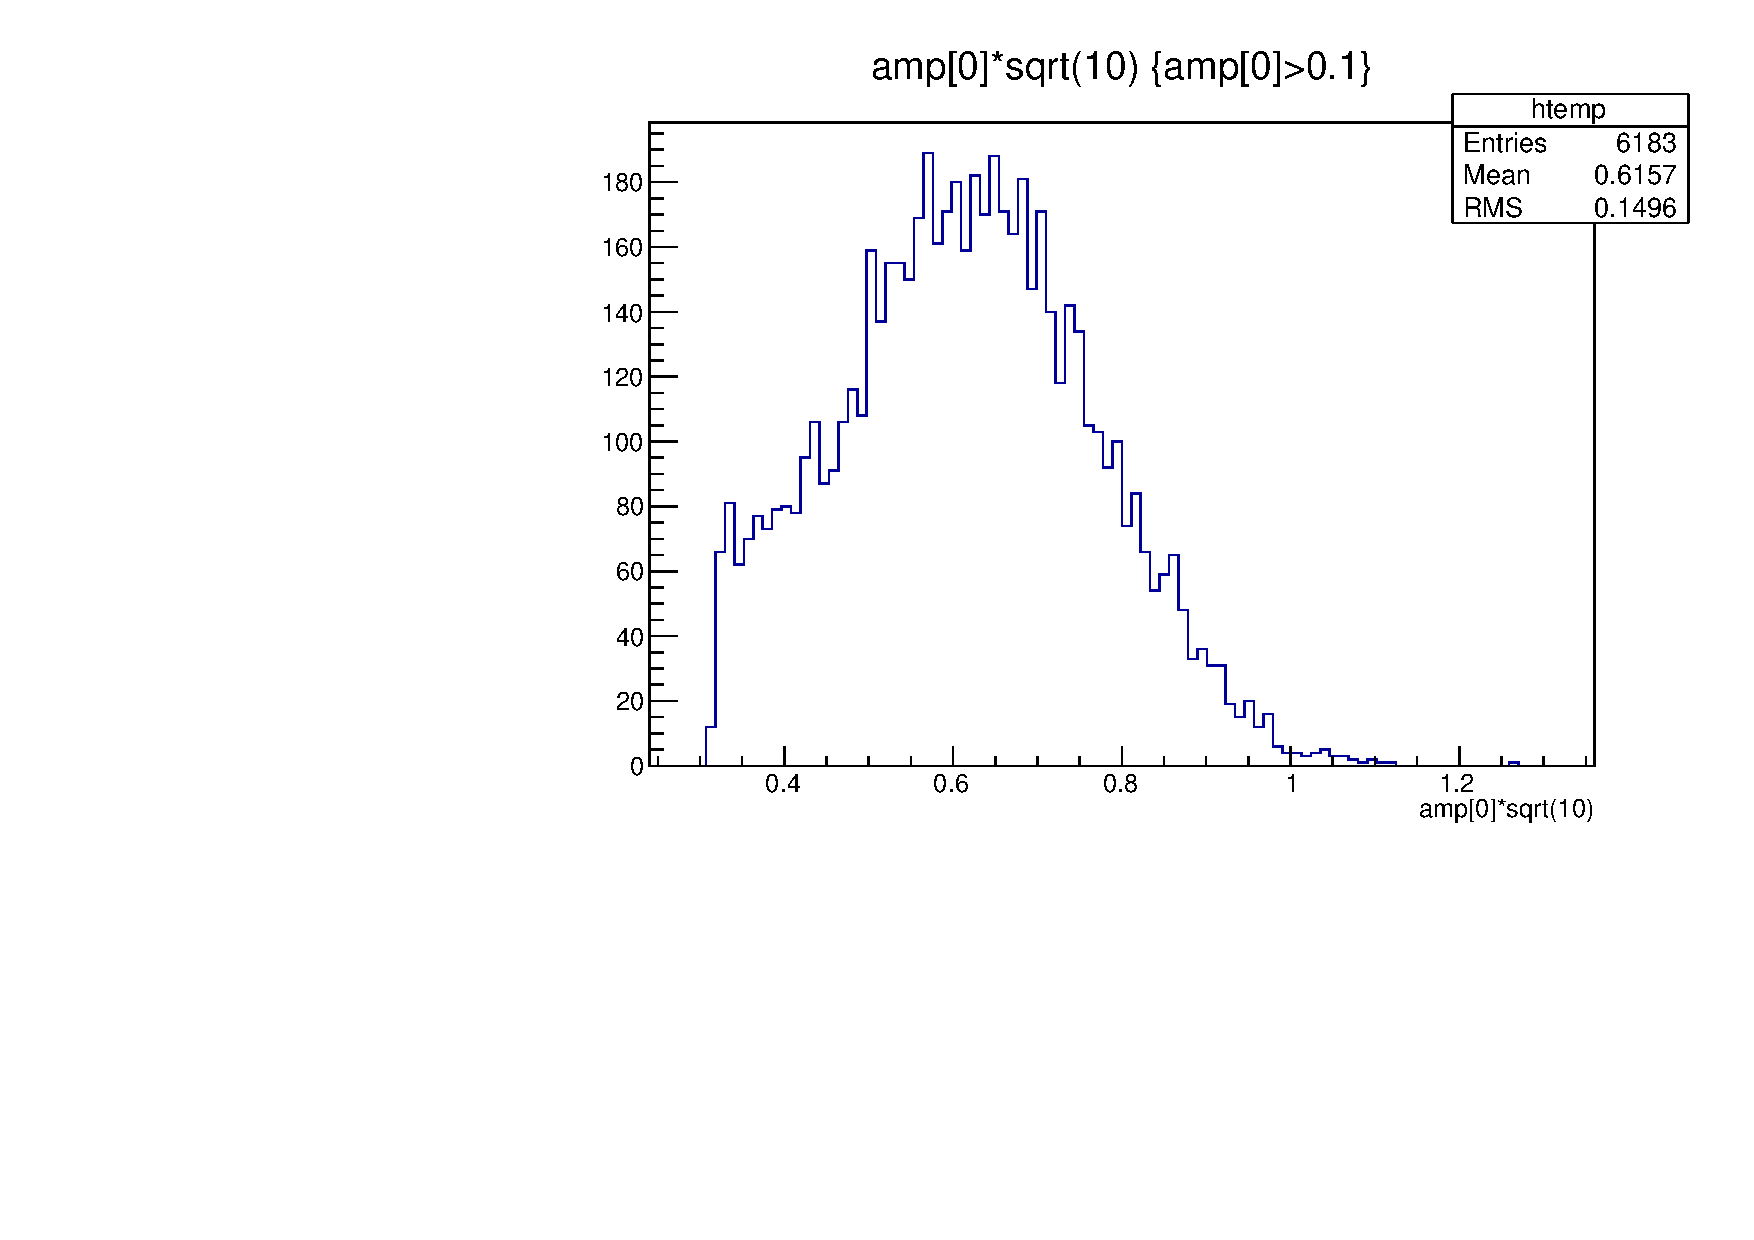
\includegraphics[width=0.49\textwidth]{AmpCut1.pdf}
	\caption{Pulse peak amplitude distribution for the Photek 240 MCP before and after the cut.
		Non-positive amplitudes represent \textit{"bad"} events.
		The $\sqrt{10}$ factor accounts for a 6 dB attenuator.}
	\label{fig:AmpCut}
\end{figure}

\begin{figure}[h]
\centering
	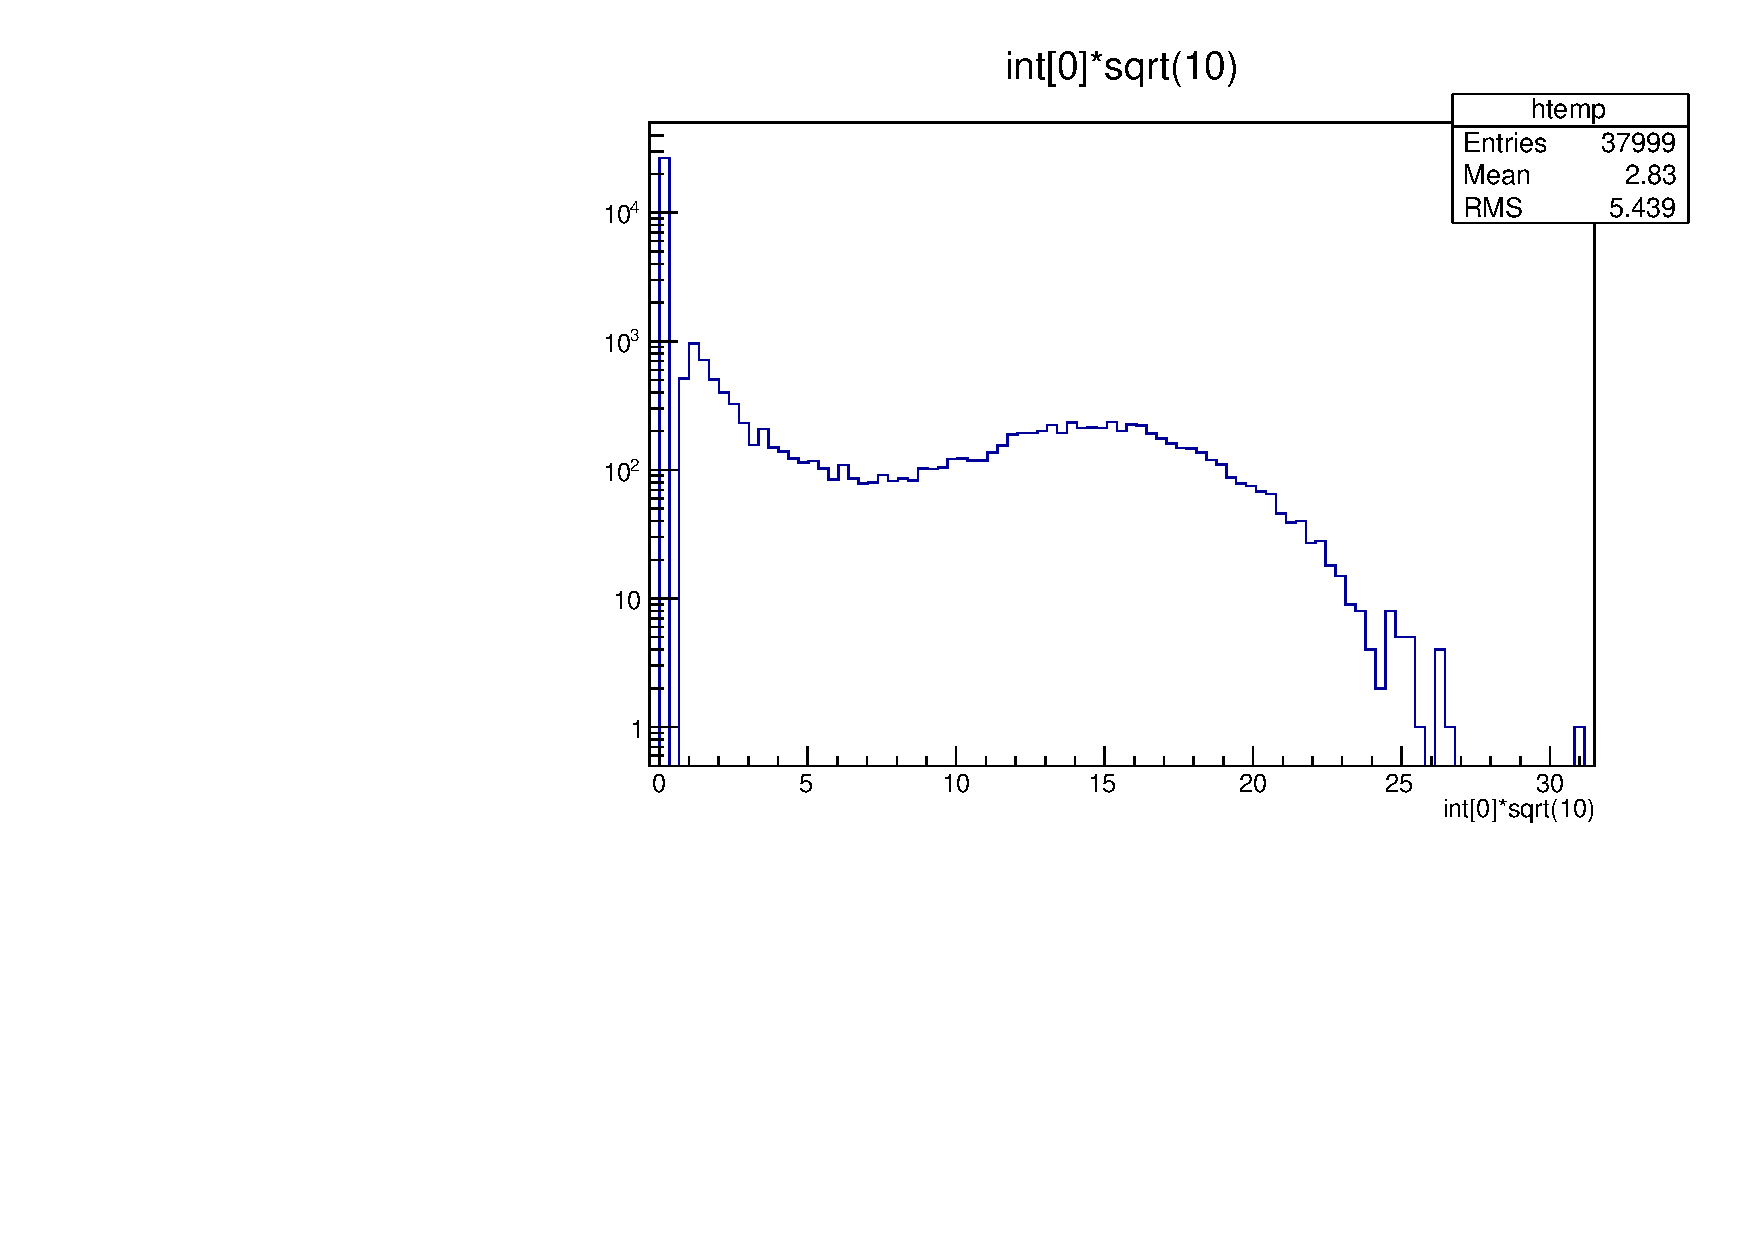
\includegraphics[width=0.49\textwidth]{ChargeCut0.pdf}
	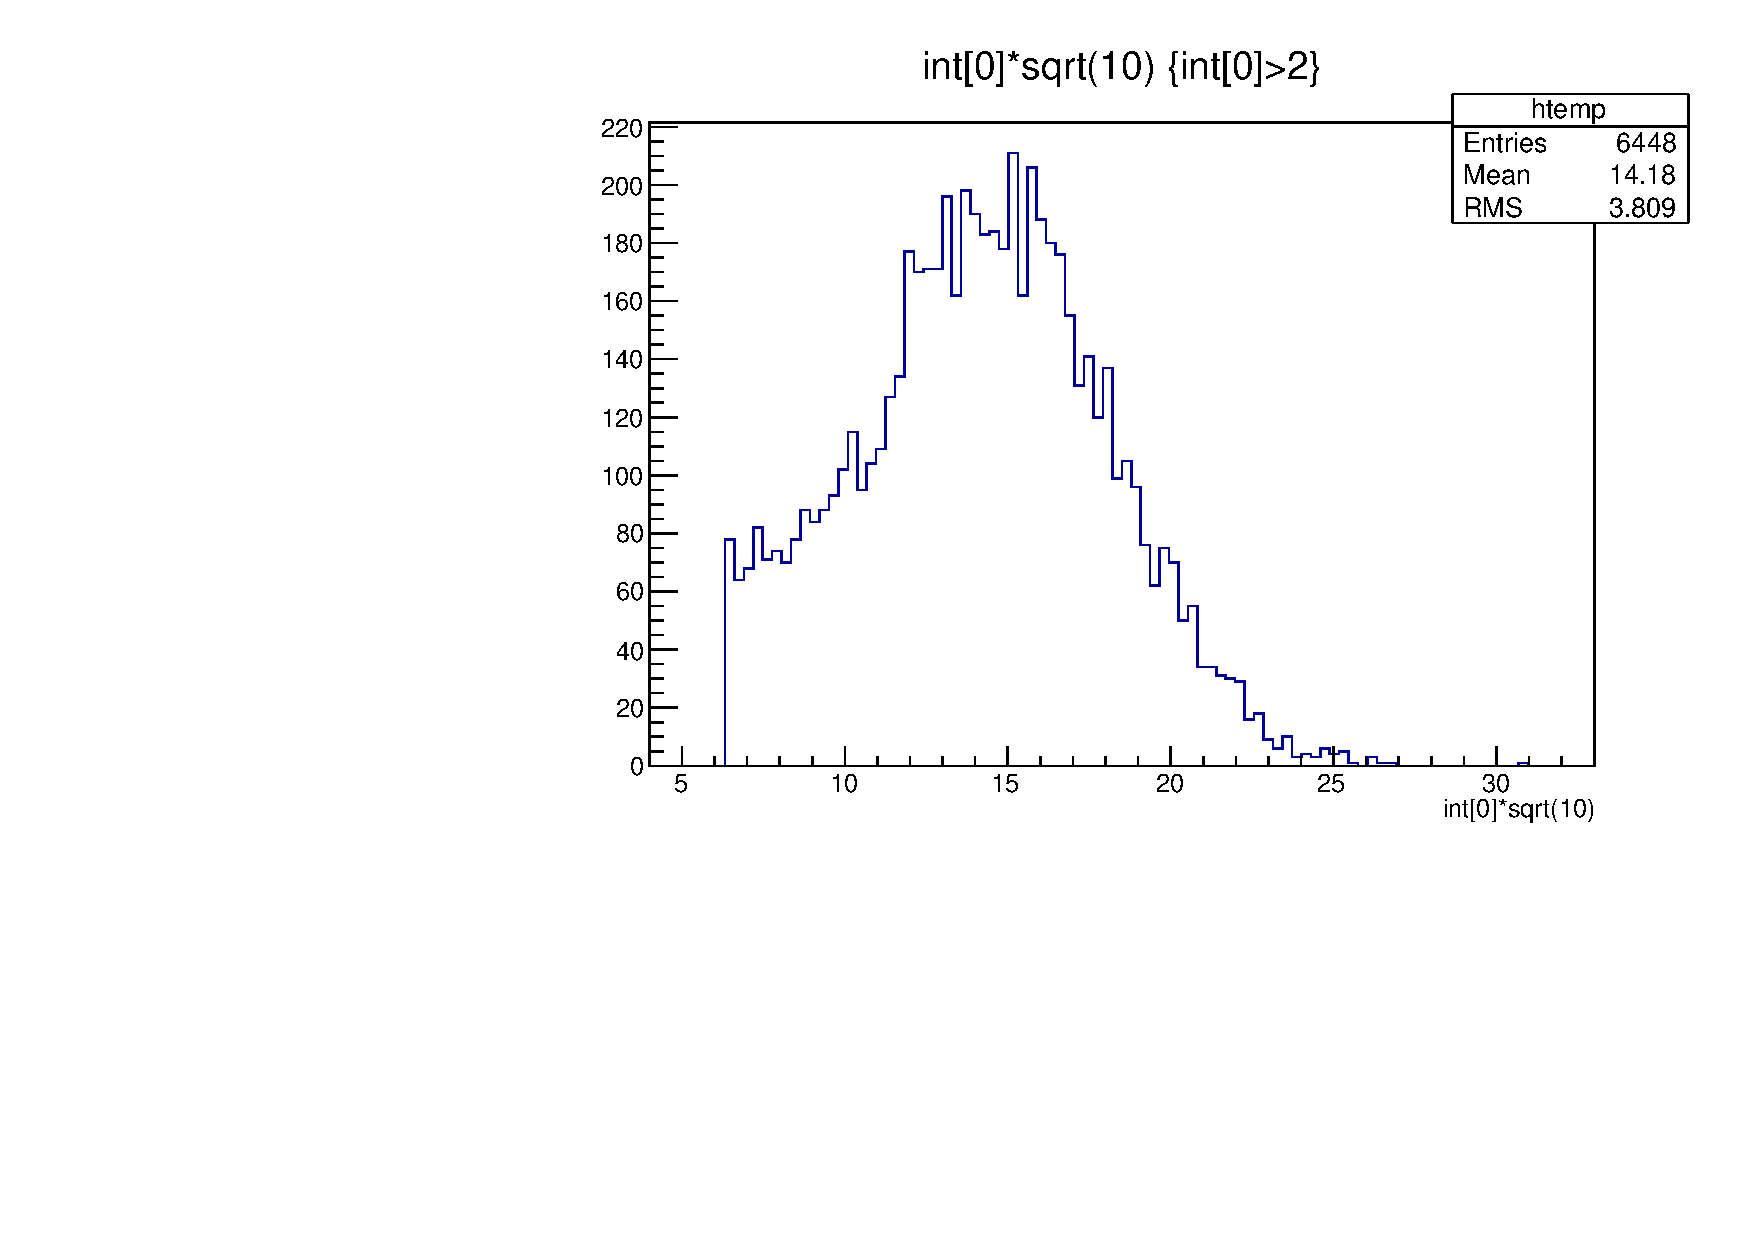
\includegraphics[width=0.49\textwidth]{ChargeCut1.pdf}
	\caption{Pulse charge distribution for the Photek 240 MCP before and after the cut.
		Zeroed charges represent events with only noise.
		The $\sqrt{10}$ factor accounts for a 6 dB attenuator.}
	\label{fig:ChargeCut}
\end{figure}

\subsection{Data Analysis: Device Combination}
The \textit{MultiDeviceStudy\_PicosilMCP} code generates many variations of TOF combination histograms. 
The simplest are the HGC center pixel and the single-channel Photonis MCP histograms (Figures \ref{fig:Center} and \ref{fig:MCP}). 
These TOFs are generated without combining the $\Delta t$ values from multiple detectors. 
There are 4 main ways that have been utilized to combine different detectors.

\subsubsection{Combination Method: Equal Weighting}
This weighting method is the most straightforward. 
If there are 2 devices which all pass the cuts, then their $\Delta t$ values are computed. 
These 2 $\Delta t$ values are then combined into a single $\Delta t$ value by computing the arithmetic average. 
This final $\Delta t$ is then used to populate the histogram. 
Mathematically, this is given by,

\[
\Delta t_{final} =
\dfrac{\Delta t_1 + \Delta t_2}{2} .
\]

It gets slightly harder to compute this $\Delta t_{final}$ when some combinations do not require that \textit{all} detectors pass the cuts, such as when trying to combine the center HGC layer pixel with the 6 inner ring pixels. 
Because many events have 3 or 4 pixels passing cuts, but only a few events have all 7 passing cuts, the $\Delta t_{final}$ is calculated at every event using whichever pixels were able to pass the cuts. 
This means the number of $\Delta t_{initial}$'s will vary with event. 
Mathematically, it can more generally be written:

\[
\Delta t_{final_i} =
\dfrac{\sum\limits_{k=1}^N \Delta t_{k_i}} {N} 
\]

for N detectors passing cuts, where $\Delta t_{k_i}$ represents the $k^{th}$ detector's TOF at event $i$.

\subsubsection{Combination Method: Event Charge Weighting}
This weighting method uses the detected event pulse charge in each device to weight each $\Delta t_{initial}$ value. 
As illustrated in Figure \ref{fig:ChargeCut1}, the pulse charge varies with event, so the relative weightings between detectors will change on an event-by-event basis. 
Mathematically, an event's charge weighting is given by,

\[
\Delta t_{final_i} =
\dfrac{\sum\limits_{k=1}^N \Delta t_{k_i} q_{k_i} }
	{\sum\limits_{k=1}^N q_{k_i} }
\]

for N detectors passing cuts, where $q_{k_i}$ represents the $k^{th}$ detector's charge at event $i$.

\subsubsection{Combination Method: Total Charge Weighting}
Whereas the event charge method weights each detector differently for different events, the total charge method weights each detector the same way over the entire run. 
Rather than use the event charge, this method sums a detector's event charge for every event in the run, and uses that value as the weighting factor. 
Mathematically,

\[
\Delta t_{final_i} =
\dfrac{\sum\limits_{k=1}^N \Delta t_{k_i} Q_k }
	{\sum\limits_{k=1}^N Q_k }
,\ \ \ \ 
Q_k = \sum_{all\ events\ i} q_{k_i}
\]

for N detectors passing cuts, where $q_{k_i}$ represents the $k^{th}$ detector's charge at event $i$.

\subsubsection{Combination Method: Charge MPV Weighting}
Like the total charge method, this method also assigns weighting factors to each detector that do not change with the event. 
This method is additionally only used within the HGC layer, for combining the TOFs of different pixels. 
Rather than being determined by the total charge detected, this method fits a Landau distribution to the charge distribution histogram of each of the inner ring pixels.
The peak -- most probable value (MPV) -- of the fit is then used as the weighting factor for the inner ring pixels. 
Because there are far more events passing cuts -- and with a higher charge -- in the center pixel, the distribution is Gaussian, and its weighting factor is the mean of a Gaussian fit.
Both types of fits are accomplished by maximizing the log-likelihood in order to avoid the biasing of the $\chi^2$ minimization fit for low-event bins.
Mathematically, this method is represented by the same formula as the total charge method, letting $Q_k$ represent the detector's MPV, instead of total charge.

\section{Time of Flight Plots}
Now that all the different combination methods have been described, understanding the resultant plots is now possible. 
In order to show results in the simplest manner, this section will only use plots coming from 1 data set with the same configuration. 
Specifically, the results in this section will all be for runs 104-116 excluding runs 111-114, which have a test beam of 32 GeV electrons, and a tungsten (W) absorber 1mm in front of the HGC layer (it may help to recall the setup from Figure \ref{fig:setup}).

Starting from the lower-level plots, Figure \ref{fig:center_MCP_104} contains the TOF histograms for the HGC center pixel and Photonis MCP.

\begin{figure}%[h]
\centering
	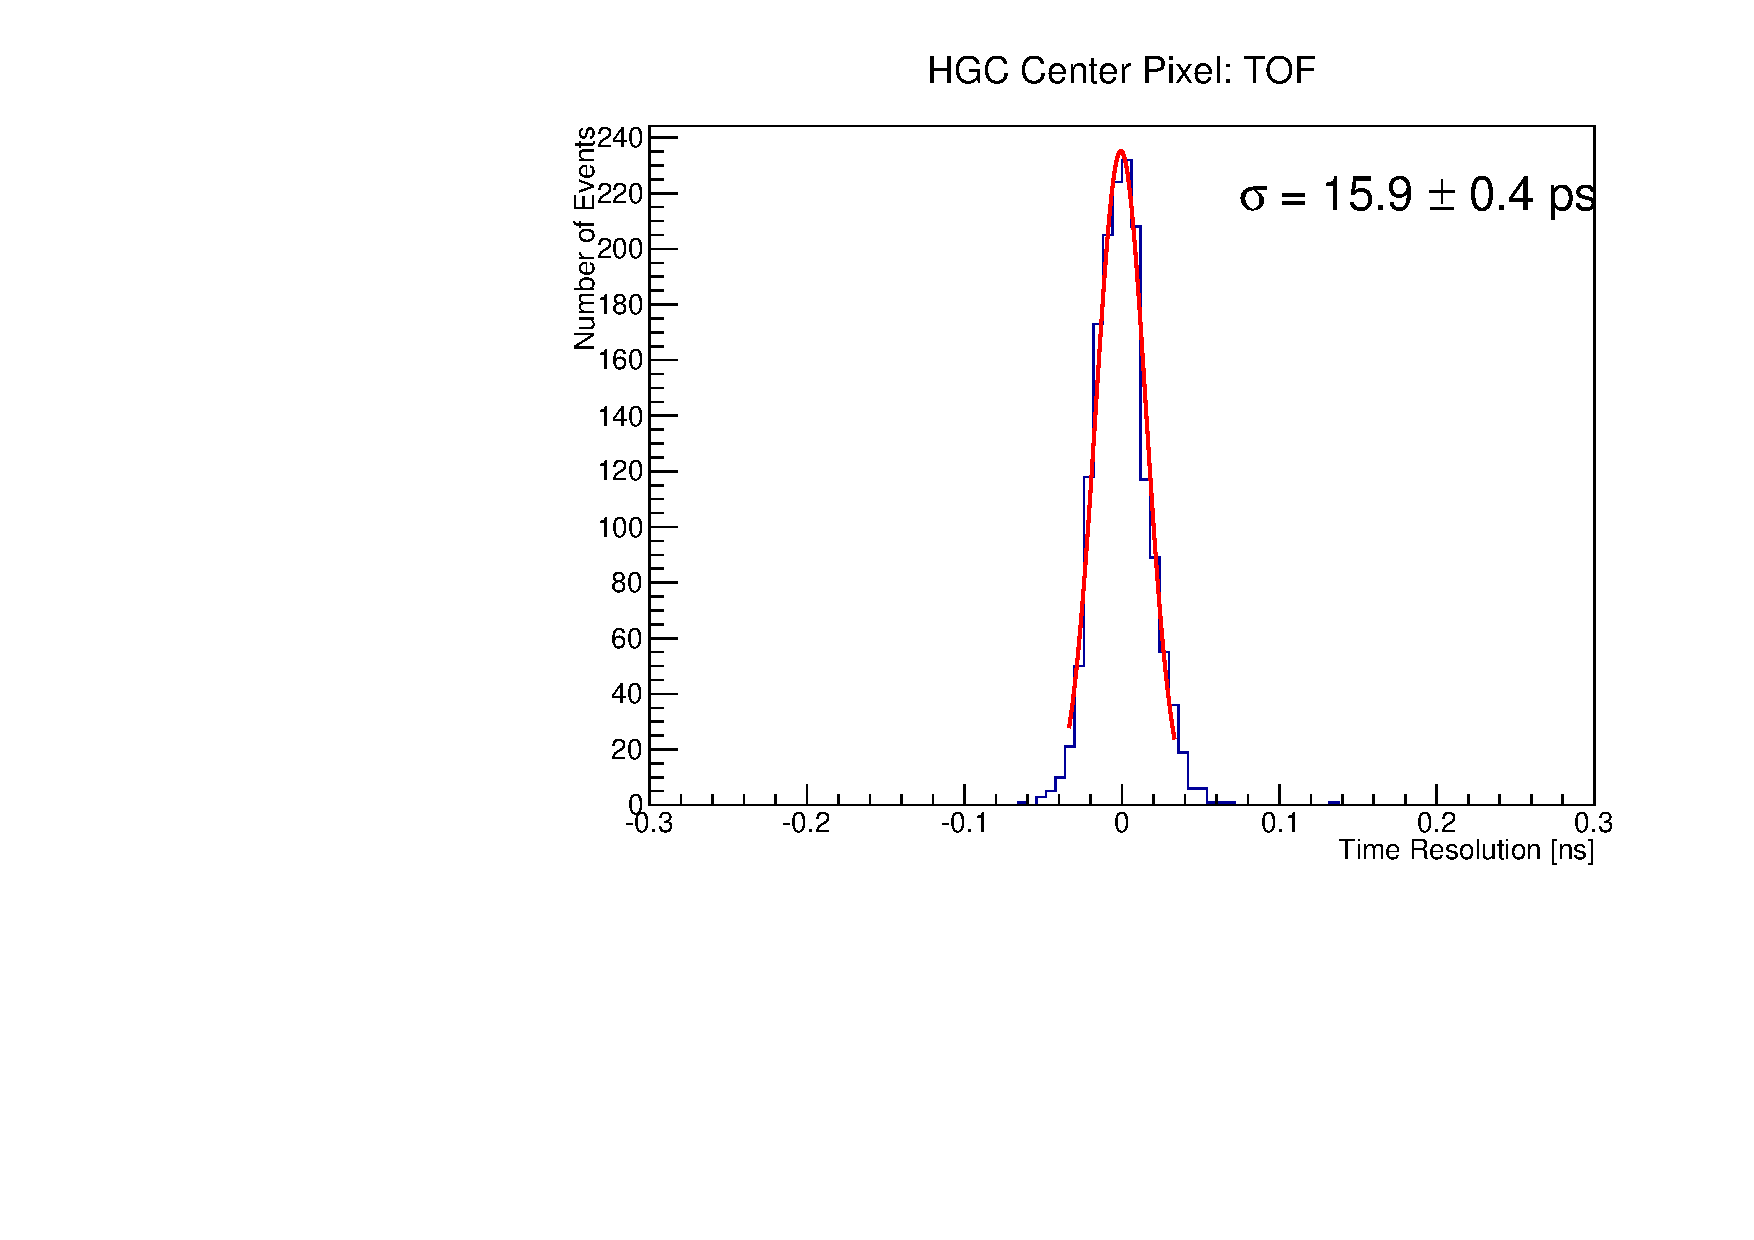
\includegraphics[width=.49\textwidth]{deltaTCenter104.pdf}
	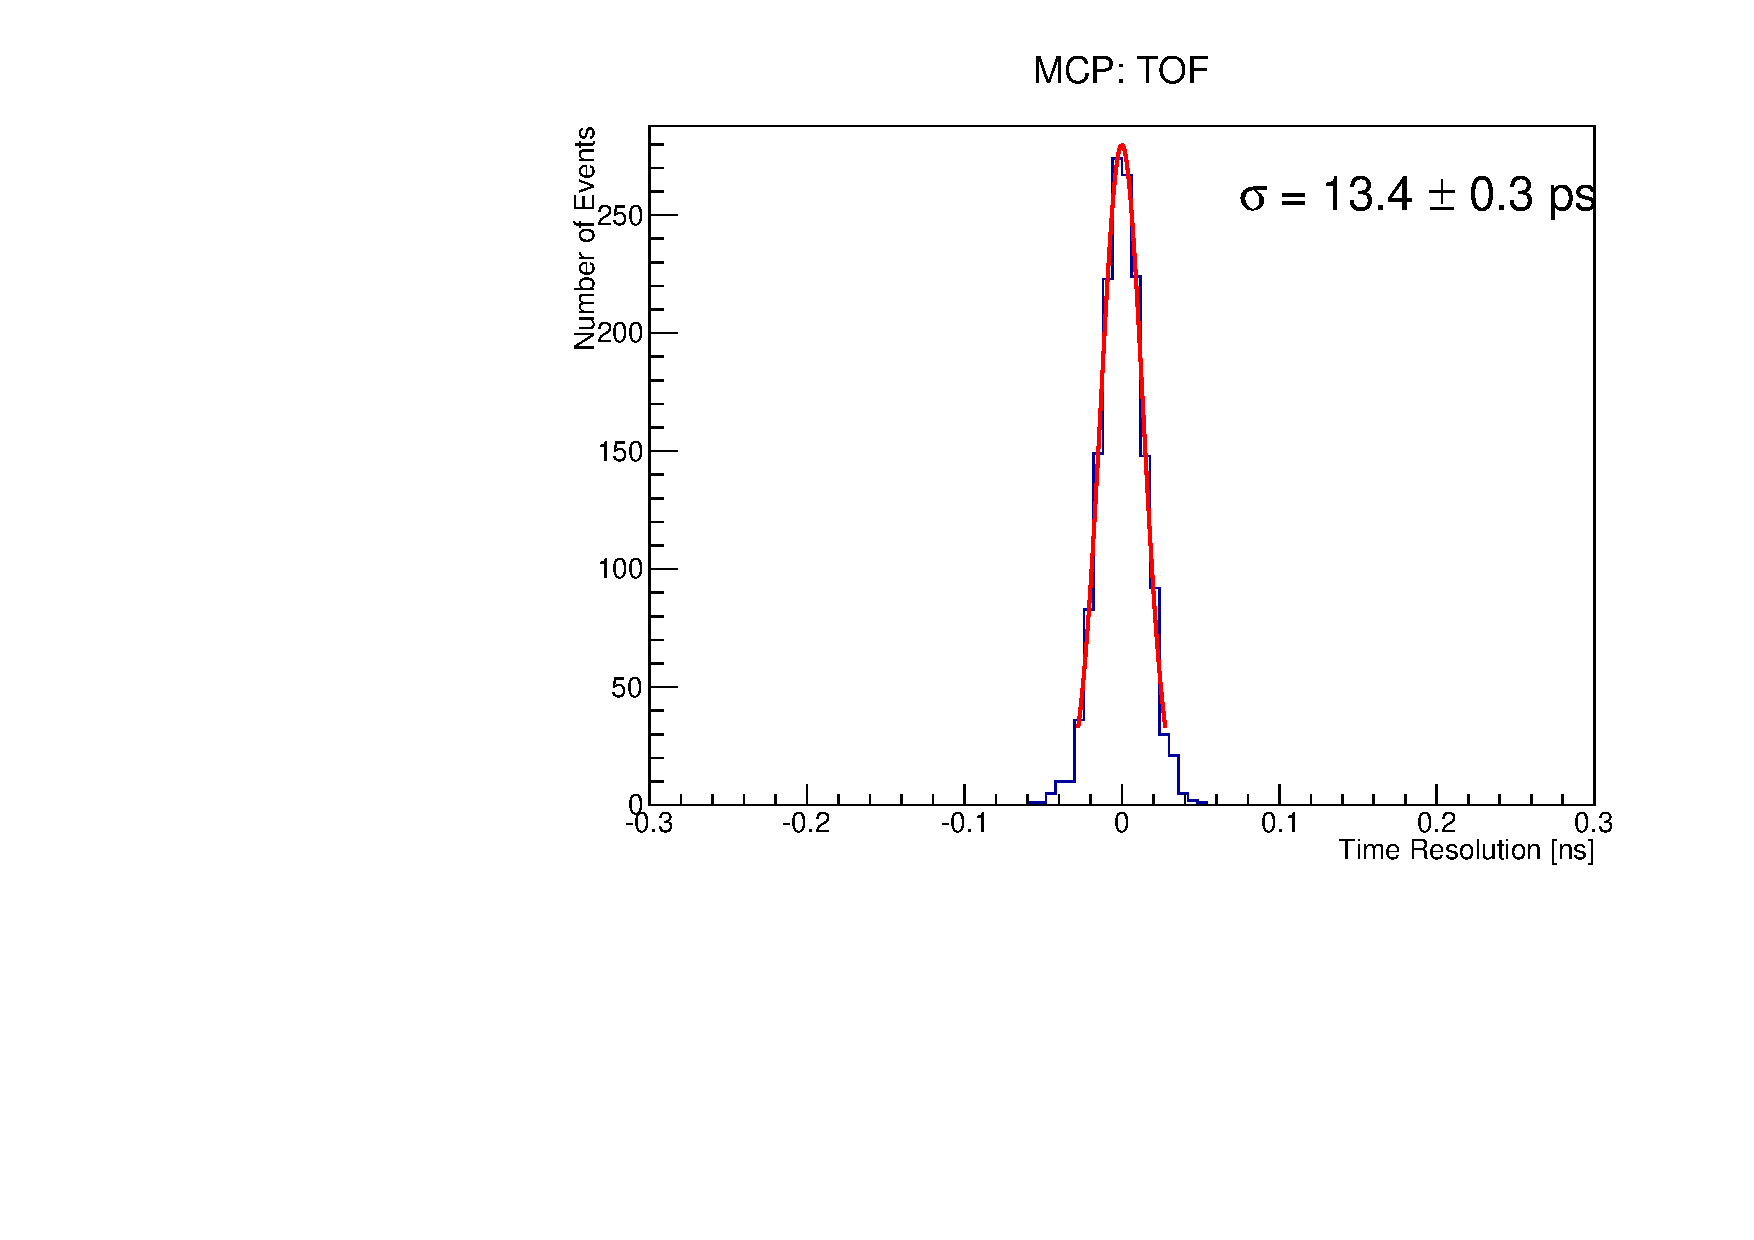
\includegraphics[width=.49\textwidth]{deltaTMCP104.pdf}
	\caption{TOF histograms of HGC center pixel and of Photonis MCP.}
	\label{fig:center_MCP_104}
\end{figure}

In order to see how the time resolution improves when adding in the inner ring pixels, Figure \ref{fig:HGC_event_total_MPV_104} contains different weighting methods based on the charge. 
Equal weighting is not used here because the center pixel has more events and a better resolution than the other pixels, so it should be weighted more heavily. 
In Figure \ref{fig:HGC_event_total_MPV_104}, there is a decrease in $\sigma$ (from 15.9 ps in Figure \ref{fig:center_MCP_104}) and thus an improvement in the time resolution for all combinations. 
Although the uncertainties in $\sigma$ are too large to be conclusive, Figure \ref{fig:HGC_event_total_MPV_104} suggests that the event charge weighting is the worst of the 3 methods.

\begin{figure}[h]
\centering
	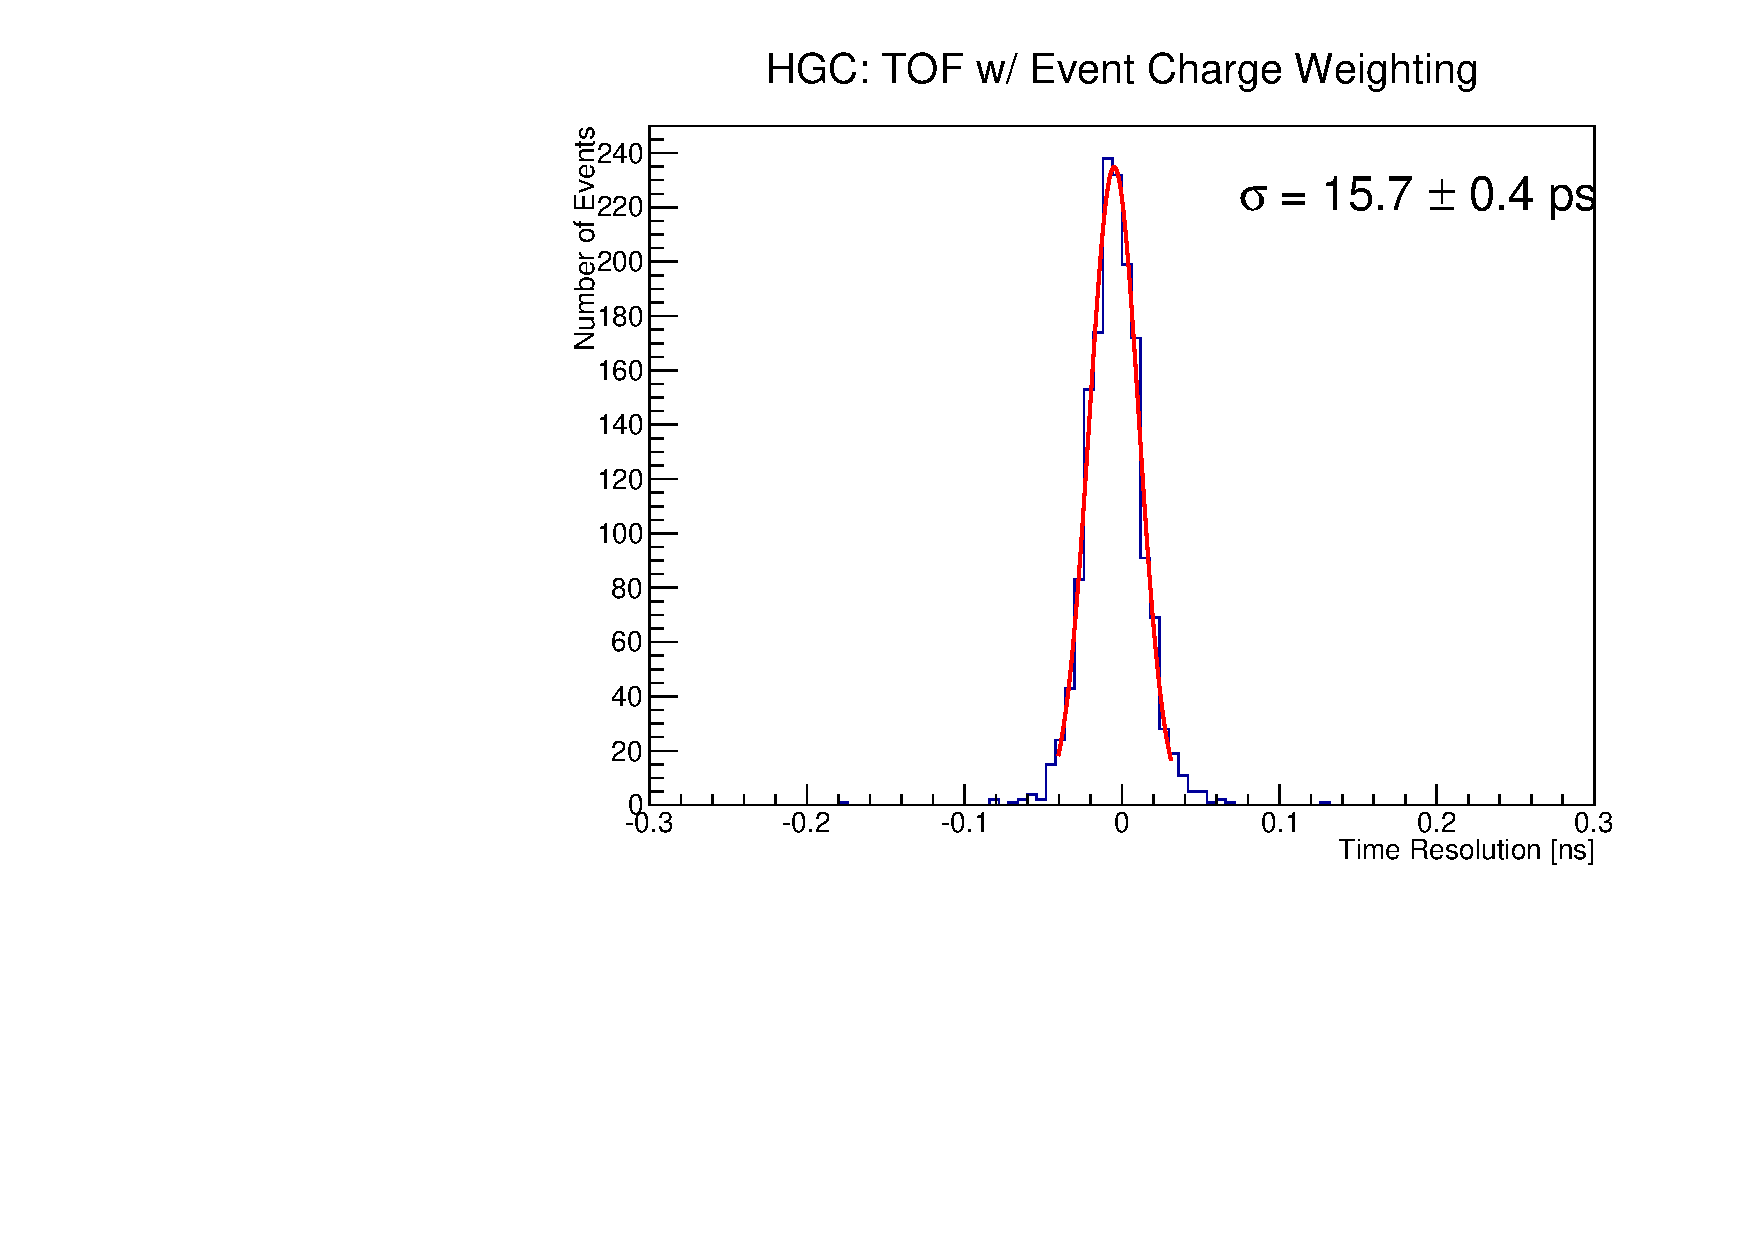
\includegraphics[width=.32\textwidth]{deltaTPicoSilEventCharge104.pdf}
	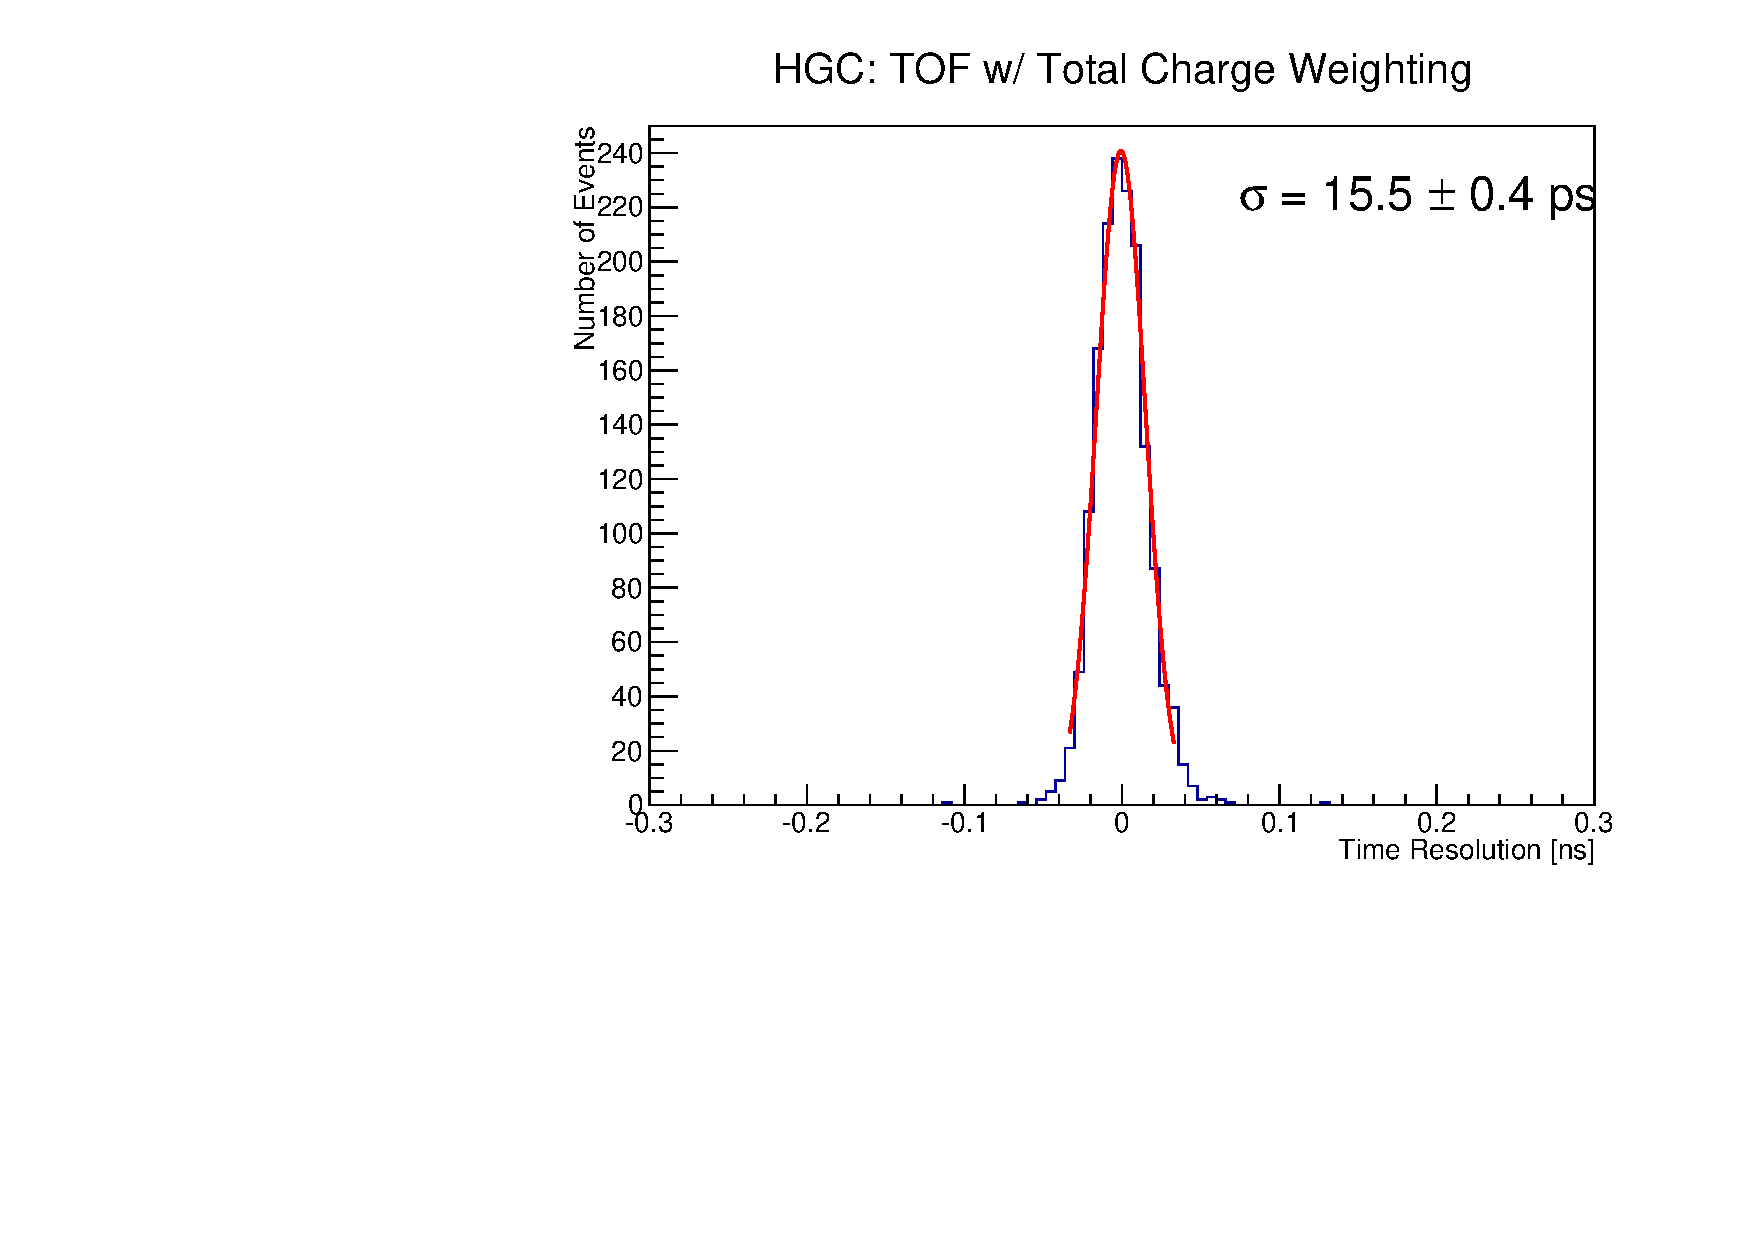
\includegraphics[width=.32\textwidth]{deltaTPicoSilTotalCharge104.pdf}
	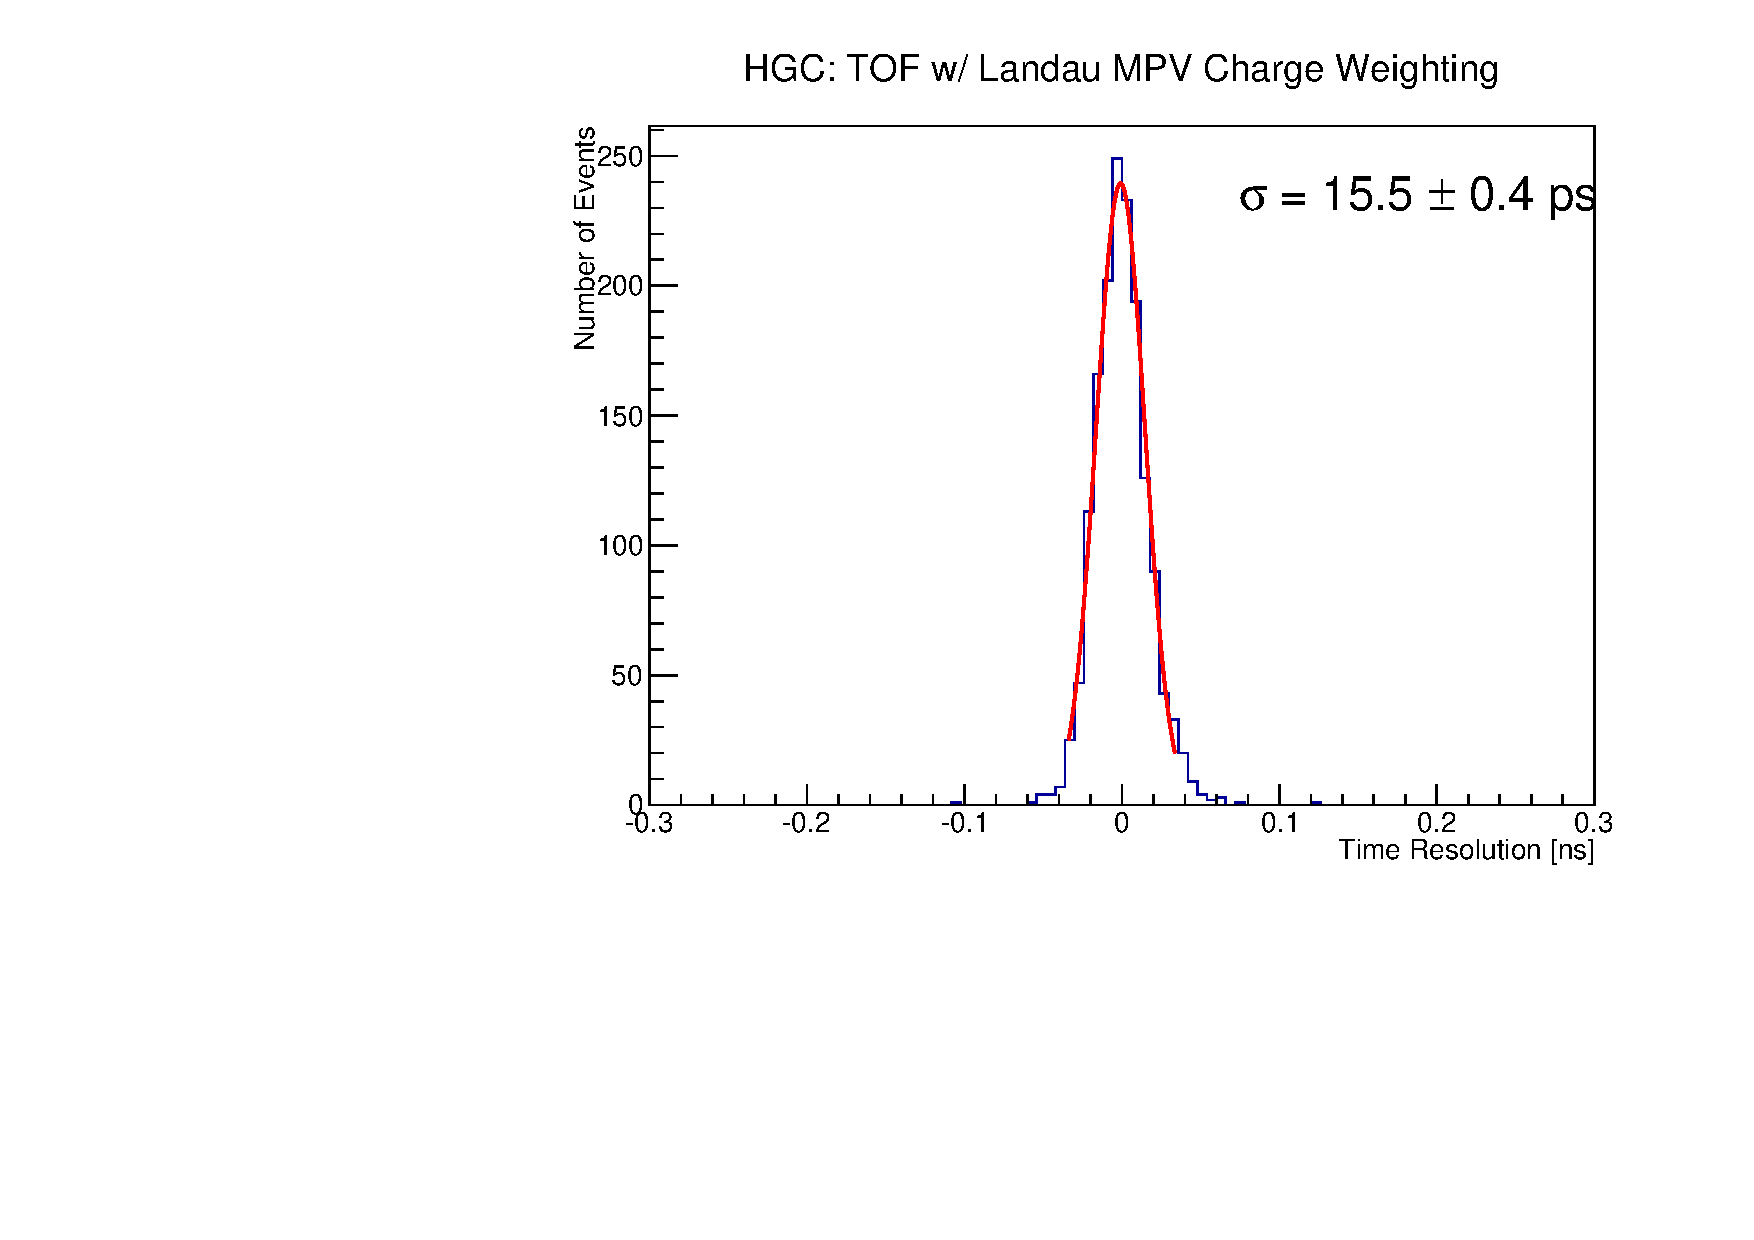
\includegraphics[width=.32\textwidth]{deltaTPicoSilLandauCharge104.pdf}
	\caption{TOF histograms of HGC pixels combined by event charge, total charge, and charge MPV.}
	\label{fig:HGC_event_total_MPV_104}
\end{figure}

The above illustrates the transverse portion of this analysis. 
For the longitudinal aspect, the $\Delta t$ values that are used to populate the HGC layer histograms in Figure \ref{fig:HGC_event_total_MPV_104} will be combined with the Photonis MCP $\Delta t$ values used to populate the right histogram in Figure \ref{fig:center_MCP_104}.
There are some basic and naive ways to combine the HGC layer with the Photonis MCP.
The first method includes assigning an equal weighting to every pixel/detector that passes the cuts.
The second method includes assigning an equal weight to all HGC pixels that pass the cuts and calculating the HGC $\Delta t$, which is then weighted equally with the Photonis $\Delta t$.
This second method can be written mathematically,

\[
\Delta t_i = \dfrac{ \Delta t_{MCP_i} }{2} + \dfrac{\sum\limits_{j=1}^N \Delta t_{HGC_{ij}} }{2\times N},\ \ \ event\ i,\ \ N\ HGC\ pixels\ passing\ cuts.
\]

The results form these two methods can be seen in Figure \ref{fig:m12}. 
Note that these two methods may seem too elementary -- especially the first method, which weights the inner ring pixels too much, and the center pixel and Photonis too little -- but they are brought up now because one of them will be used later in a smarter way. 
Here however, both methods (utilizing 8 detectors) gave a worse time resolution than just the central HGC pixel.	

\begin{figure}[h]
\centering
	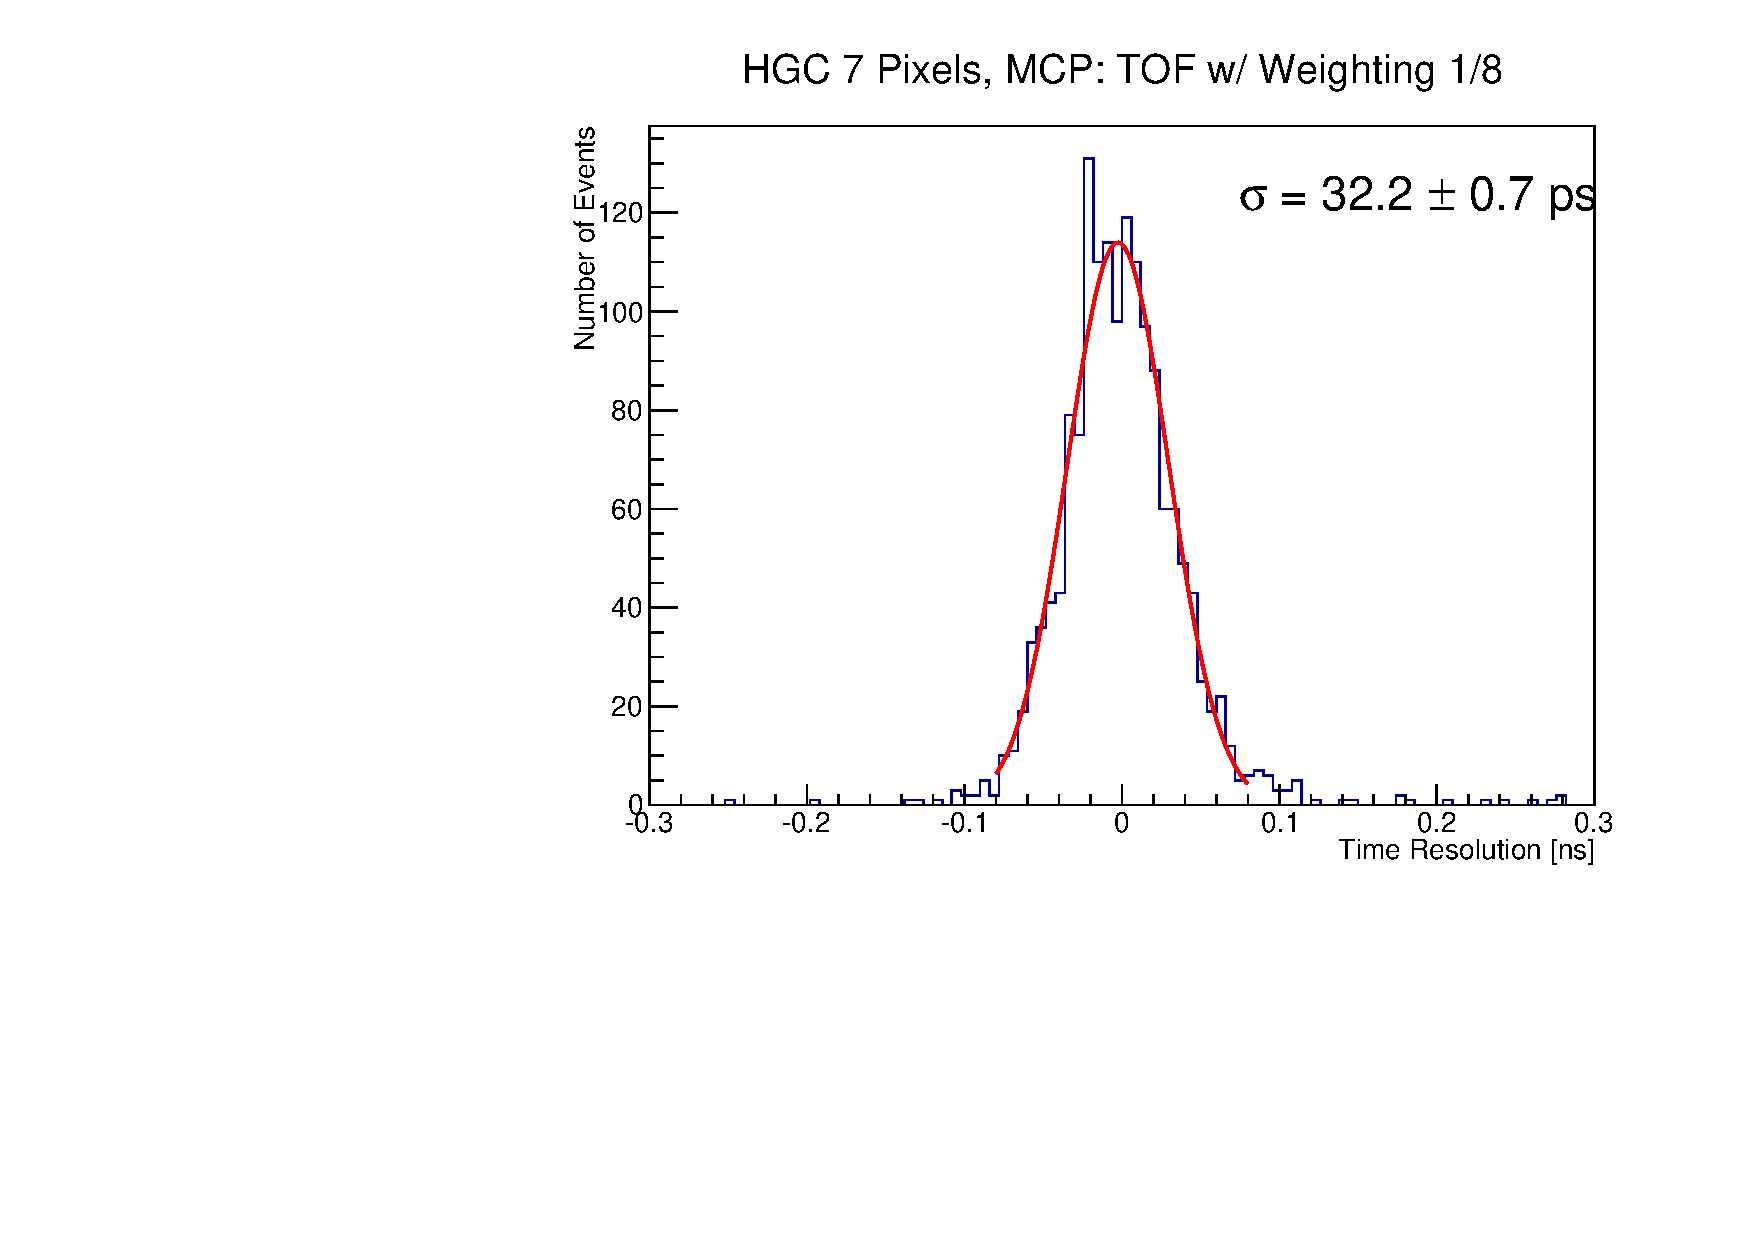
\includegraphics[width=.49\textwidth]{deltaT_PicoSil_MCP_Equal104.pdf}
	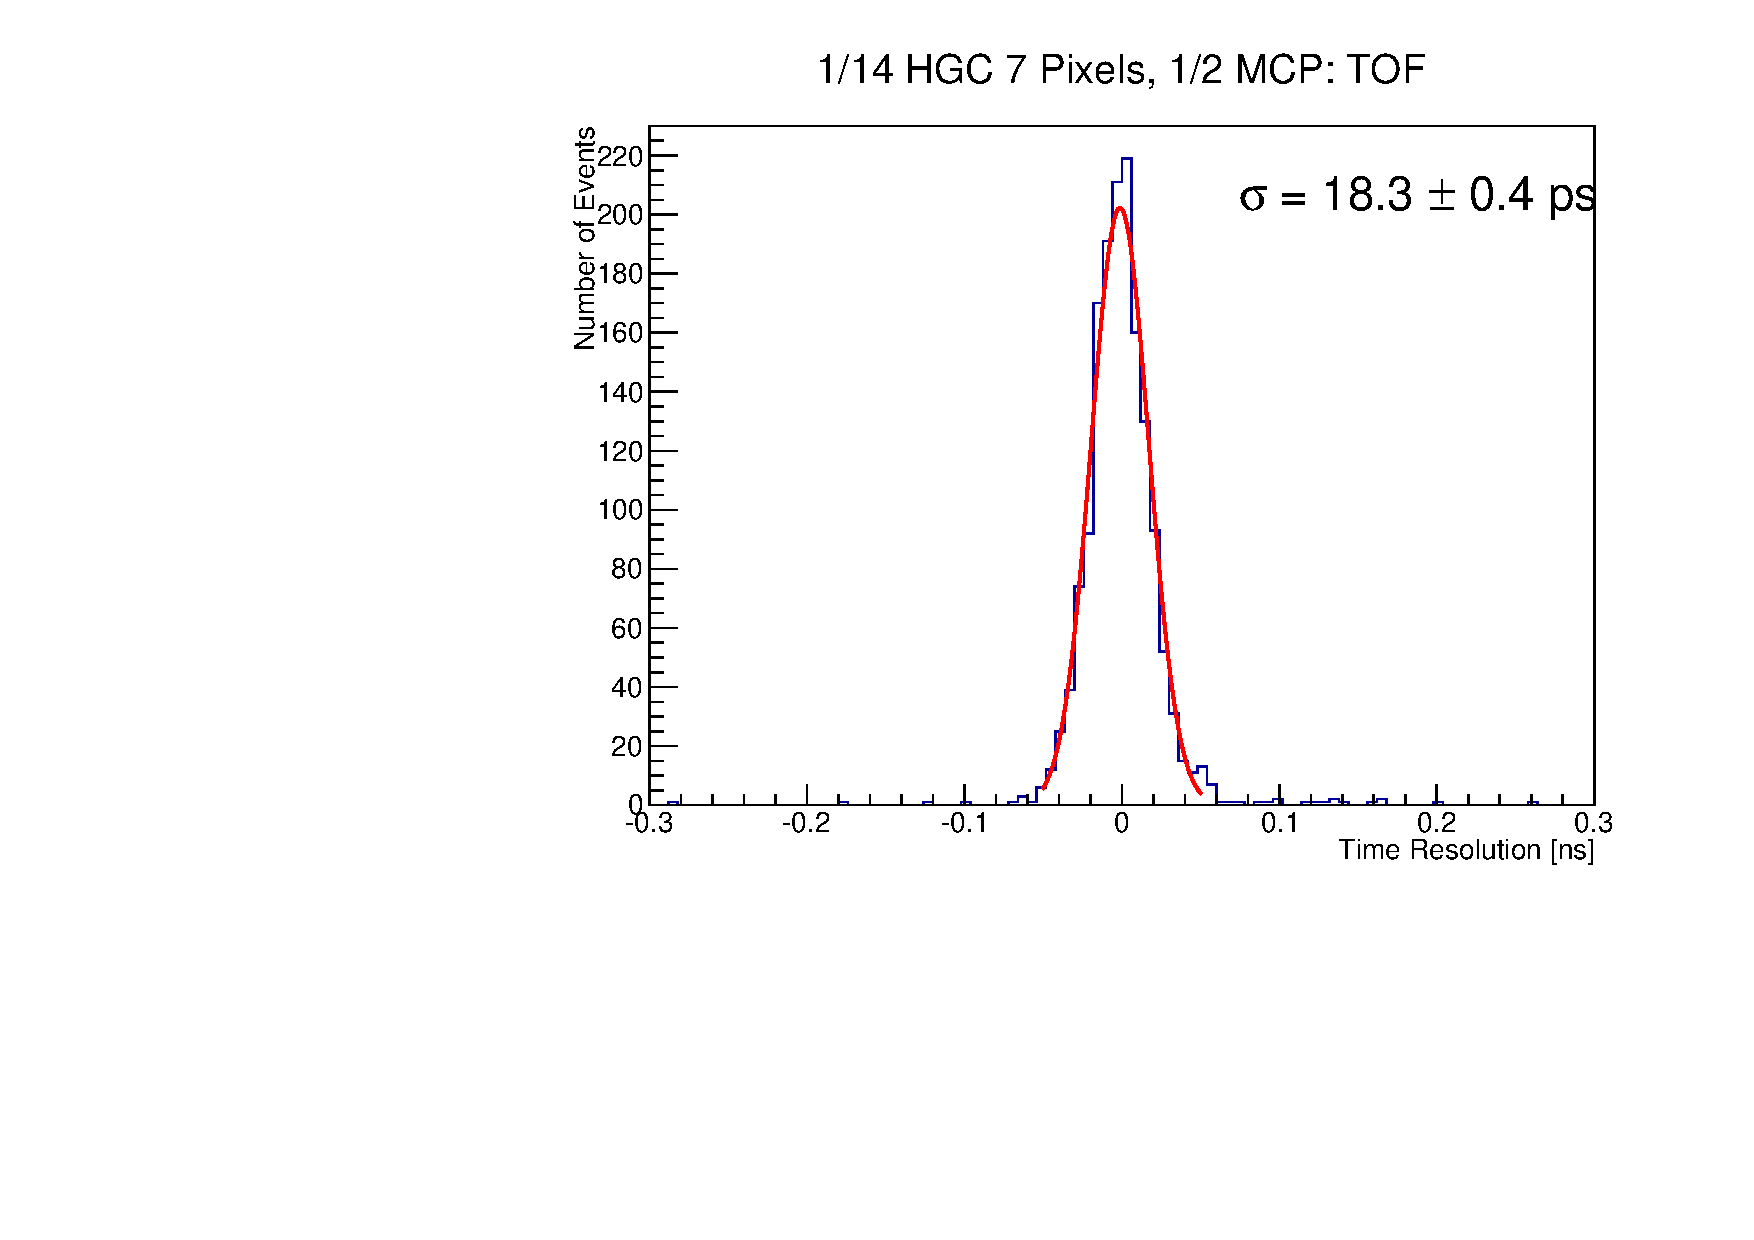
\includegraphics[width=.49\textwidth]{deltaT_PicoSilEqual_MCP_Equal104.pdf}
	\caption{Implementation of basic methods 1 (left) and 2 (right) as described in the text. }
	\label{fig:m12}
\end{figure}

Smarter ways to combine the HGC layer with the Photonis MCP includes weighting each pixel and the Photonis by their event or total charge. 
Mathematically, these methods would be given by,

\[
\Delta t_i = 
\dfrac{ \Delta t_{MCP_i} q_{MCP_i} +
	\sum\limits_{all\ pixels} \Delta t_{HGC_i} q_{HGC_i} }
	{ q_{MCP_i} +
	\sum\limits_{all\ pixels} q_{HGC_i} }
\]

\[
\Delta t_i = 
\dfrac{ \Delta t_{MCP_i} Q_{MCP} +
	\sum\limits_{all\ pixels} \Delta t_{HGC_i} Q_{HGC} }
	{ Q_{MCP} +
	\sum\limits_{all\ pixels} Q_{HGC} }
\]

Figure \ref{fig:HGC_MCP_event_total_104} gives the TOF histograms using these combination methods.

\begin{figure}[h]
\centering
	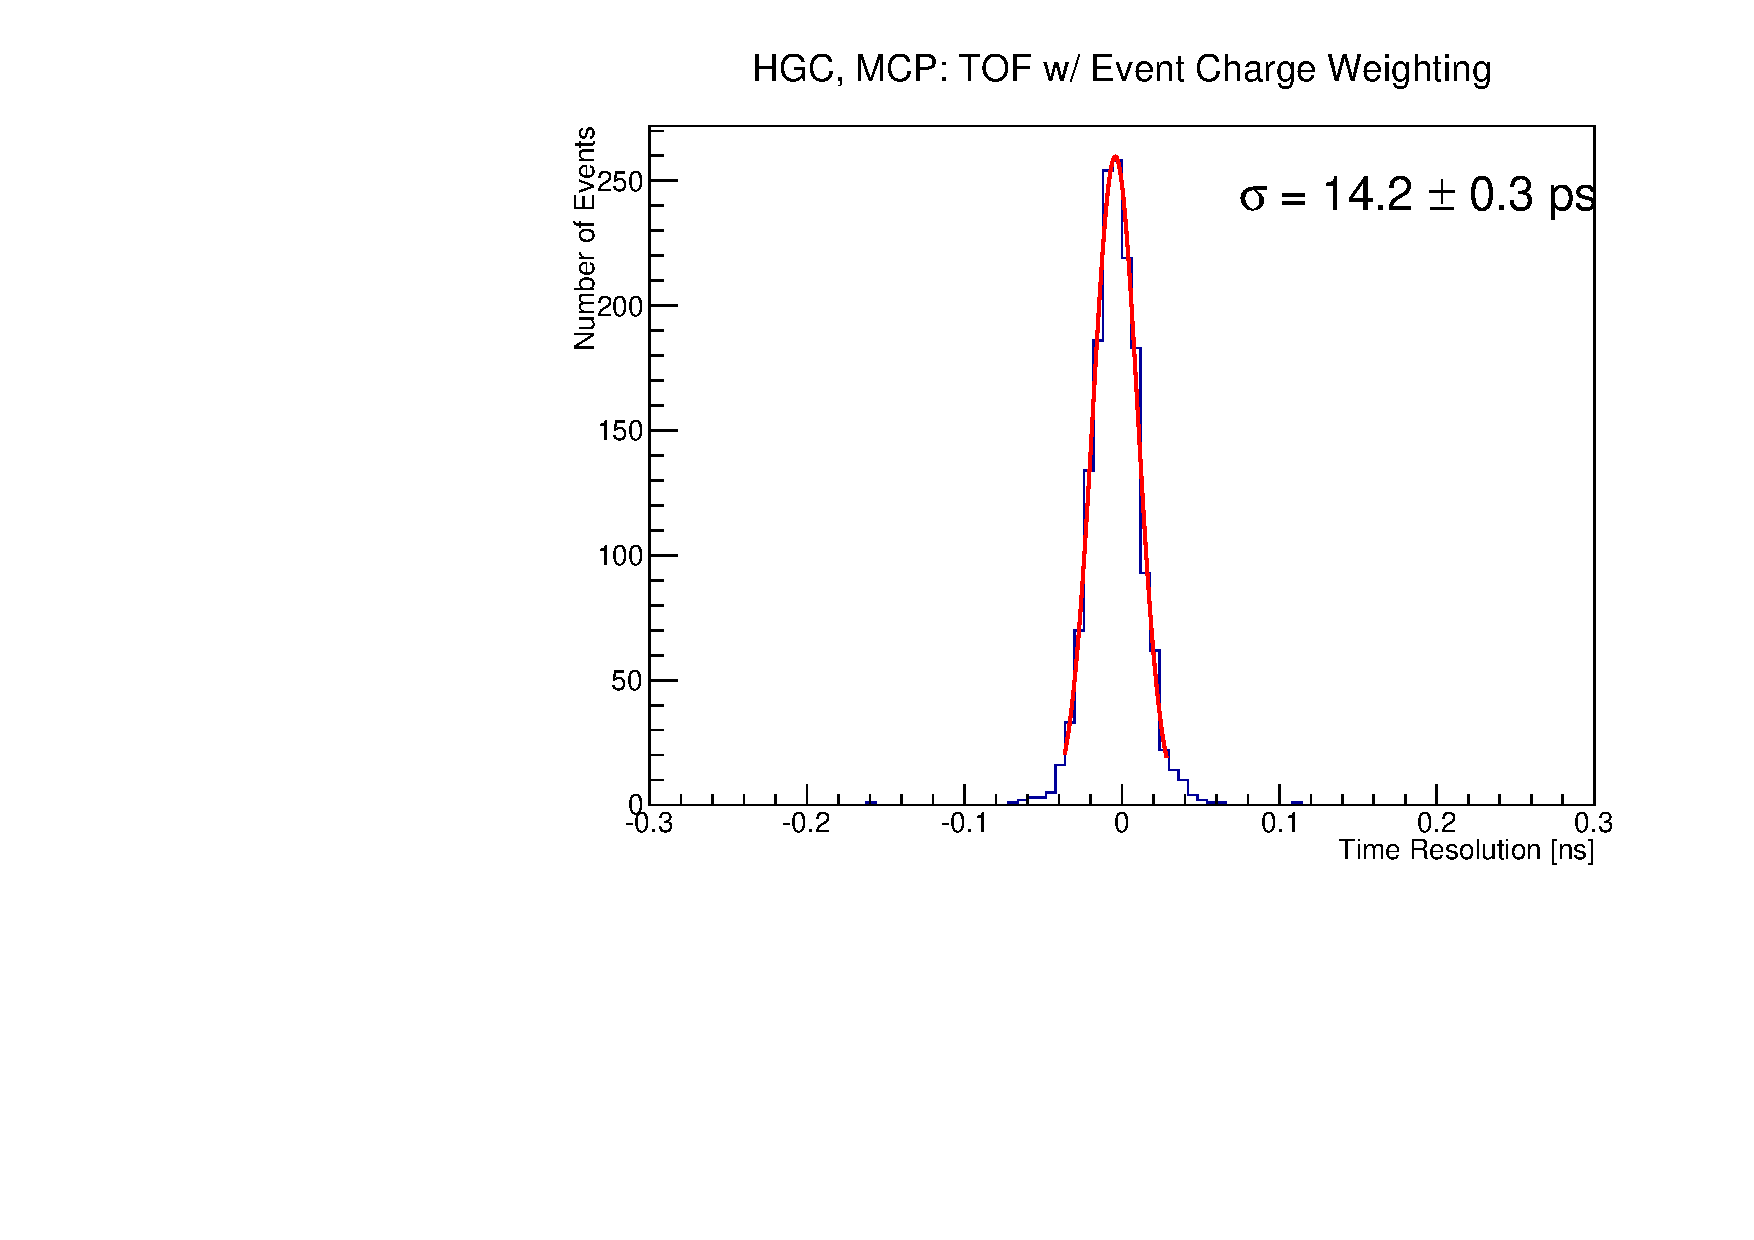
\includegraphics[width=.49\textwidth]{deltaT_PicoSil_MCP_EventCharge104.pdf}
	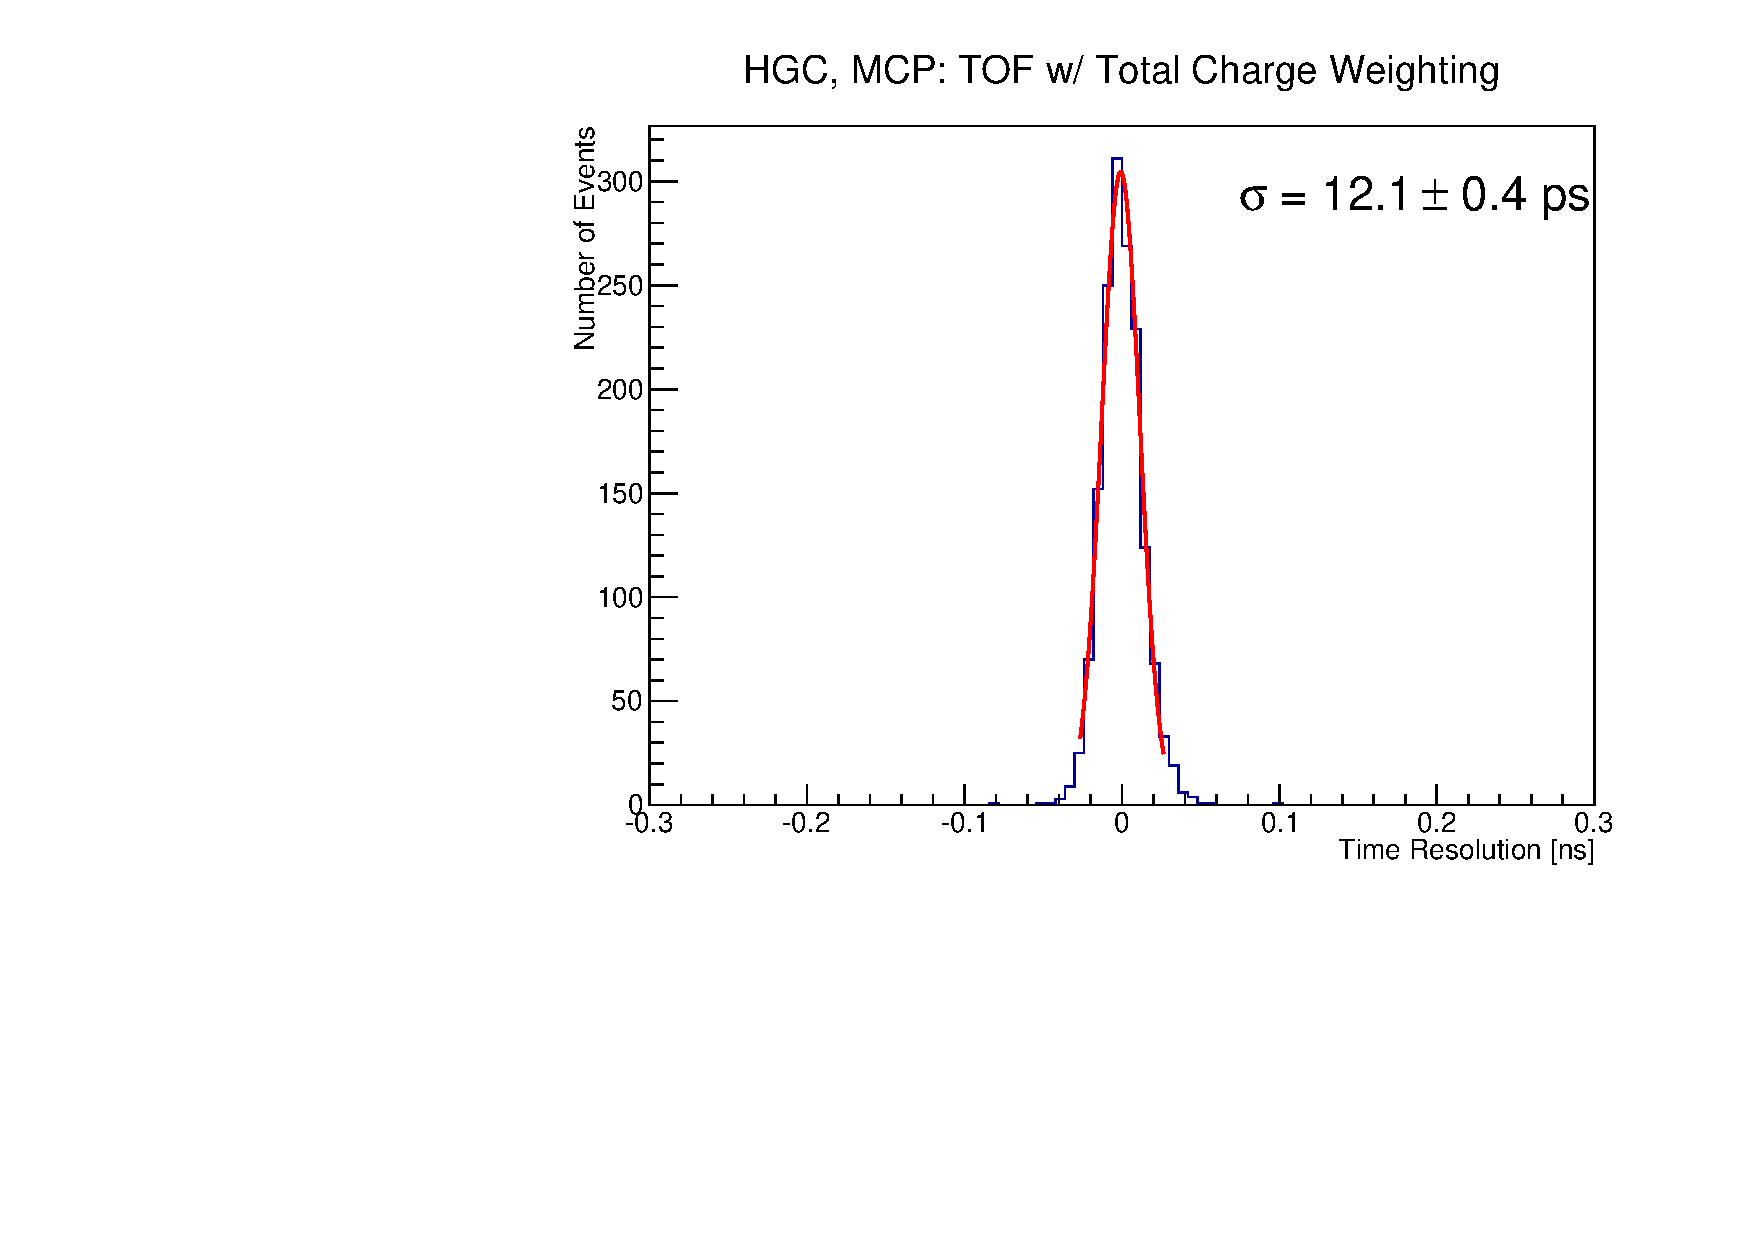
\includegraphics[width=.49\textwidth]{deltaT_PicoSil_MCP_TotalCharge104.pdf}
	\caption{TOF histograms of the HGC pixels and Photonis MCP, using event (left) and total (right) charge weighting. }
	\label{fig:HGC_MCP_event_total_104}
\end{figure}



\_\_\_\_\_\_\_\_\_\_\_\_\_\_\_\_\_\_\_\_\_\_\_\_\_\_\_\_\_\_\_\_\_\_\_\_\_\_\_\_\_\_\_\_\_\_\_\_\_\_\_\_\_\_\_\_\_\_\_\_\_\_\_\_\_\_\_\_\_\_\_\_\_\_\_\_\_\_\_\_\_\_\_\_\_\_\_\_\_\_\_\_\_\_\_\_

\_\_\_\_\_\_\_\_\_\_\_\_\_\_\_\_\_\_\_\_\_\_\_\_ Stopped my revisions here \_\_\_\_\_\_\_\_\_\_\_\_\_\_\_\_\_\_\_\_\_\_\_\_

\_\_\_\_\_\_\_\_\_\_\_\_\_\_\_\_\_\_\_\_\_\_\_\_\_\_\_\_\_\_\_\_\_\_\_\_\_\_\_\_\_\_\_\_\_\_\_\_\_\_\_\_\_\_\_\_\_\_\_\_\_\_\_\_\_\_\_\_\_\_\_\_\_\_\_\_\_\_\_\_\_\_\_\_\_\_\_\_\_\_\_\_\_\_\_\_

Another histogram (Figure \ref{fig:CenterMCPEqual}) is the average value of the center pixel and the MCP $\Delta t$ at every event. 
Figure 4 adds in the other 6 pixels of the inner ring of the HGC layer, and weights everything by taking the arithmetic average of the $\Delta t$’s for the pixels that passed the cuts.

	The histogram  in Figure 5 averages all 7 of the HGC pixel $\Delta t$’s equally, and then averages that value with the MCP:

\[
\Delta t_i = \dfrac{ \Delta t_{MCP_i} }{2} + \dfrac{\sum\limits_{j=1}^N \Delta t_{HGC_{ij}} }{2\times N},\ \ \ event\ i,\ \ N\ HGC\ pixels\ passing\ cuts
\]

However, the last two combinations (Figures 4/5) are not the best ways to combine the pixels in the HGC. 
Due to the electromagnetic nature of the particle beam, the shower spreads out as it evolves, so more particles will pass through some of the pixels than others \cite{P2}. 
As it turns out, the center pixel detects significantly more charge than the others, so it should be weighted more. 
There are two ways to weight the HGC combination by the charge: (1) At every event, compute the relative charge in every pixel and use that as the weighting factor, or (2) loop over all events and find the total charge deposited in a pixel over the entire run, then do this for every pixel and use those values as the weights. 
The first method will weigh the pixels differently at every event, whereas the second method will weigh the pixels the same way for every event.

Without including the MCP, two other histograms (Figures 6 and 7) plot the event $\Delta t$’s using the event charge and total run charge weightings:

\[
\Delta t_i = 
\dfrac{ \sum\limits_{all\ pixels} \Delta t_{HGC_i} q_{HGC_i} }
	{ \sum\limits_{all\ pixels} q_{HGC_i} }
,\ \ \ event\ i
,\ \ event\ pixel\ charge\ q_i
\]

\[
\Delta t_i = 
\dfrac{ \sum\limits_{all\ pixels} \Delta t_{HGC_i} Q_{HGC} }
	{ \sum\limits_{all\ pixels} Q_{HGC} }
,\ \ \ event\ i
,\ \ total\ run\ pixel\ charge\ Q
\]

Utilizing these weighting methods, two other histograms (Figures 8 and 9) weight every pixel in the HGC and the MCP by their event charge and their total charge:

\[
\Delta t_i = 
\dfrac{ \Delta t_{MCP_i} q_{MCP_i} +
	\sum\limits_{all\ pixels} \Delta t_{HGC_i} q_{HGC_i} }
	{ q_{MCP_i} +
	\sum\limits_{all\ pixels} q_{HGC_i} }
\]

\[
\Delta t_i = 
\dfrac{ \Delta t_{MCP_i} Q_{MCP} +
	\sum\limits_{all\ pixels} \Delta t_{HGC_i} Q_{HGC} }
	{ Q_{MCP} +
	\sum\limits_{all\ pixels} Q_{HGC} }
\]

These \textit{would} be the best ways to combine everything if we could guarantee that a particle of a specific energy detected in the HGC would give the same charge as a detection in the MCP. 
However, since the HGC and the MCP have different gains that are not known, a better way to weight the histograms would be to do either an event charge or total run charge weighting for the HGC $\Delta t$ and then weight that and the MCP $\Delta t$ each by half (Figures 10 and 11).

\[
\Delta t_i = 
\dfrac{
\left[ \sum\limits_{all\ pixels} \Delta t_{HGC_i} q_{HGC_i}
\div
\sum\limits_{all\ pixels} q_{HGC_i}
\right]
+ \Delta t_{MCP_i} 
} {2}
\]

\[
\Delta t_i = 
\dfrac{
\left[ \sum\limits_{all\ pixels} \Delta t_{HGC_i} Q_{HGC}
\div
\sum\limits_{all\ pixels} Q_{HGC}
\right]
+ \Delta t_{MCP_i} 
} {2}
\]

I have still yet to determine which of the event charge or total run charge weightings is optimal. 
Note: my code fits every histogram 2$\times$RMS around each peak with a Gaussian.

\textit{ The following figures were generated through running my analysis code on runs 65-83. }

%%% INCLUDE 9 FIGURES %%%

\begin{figure}
\centering
\begin{minipage}[t]{.49\textwidth}
	\centering
	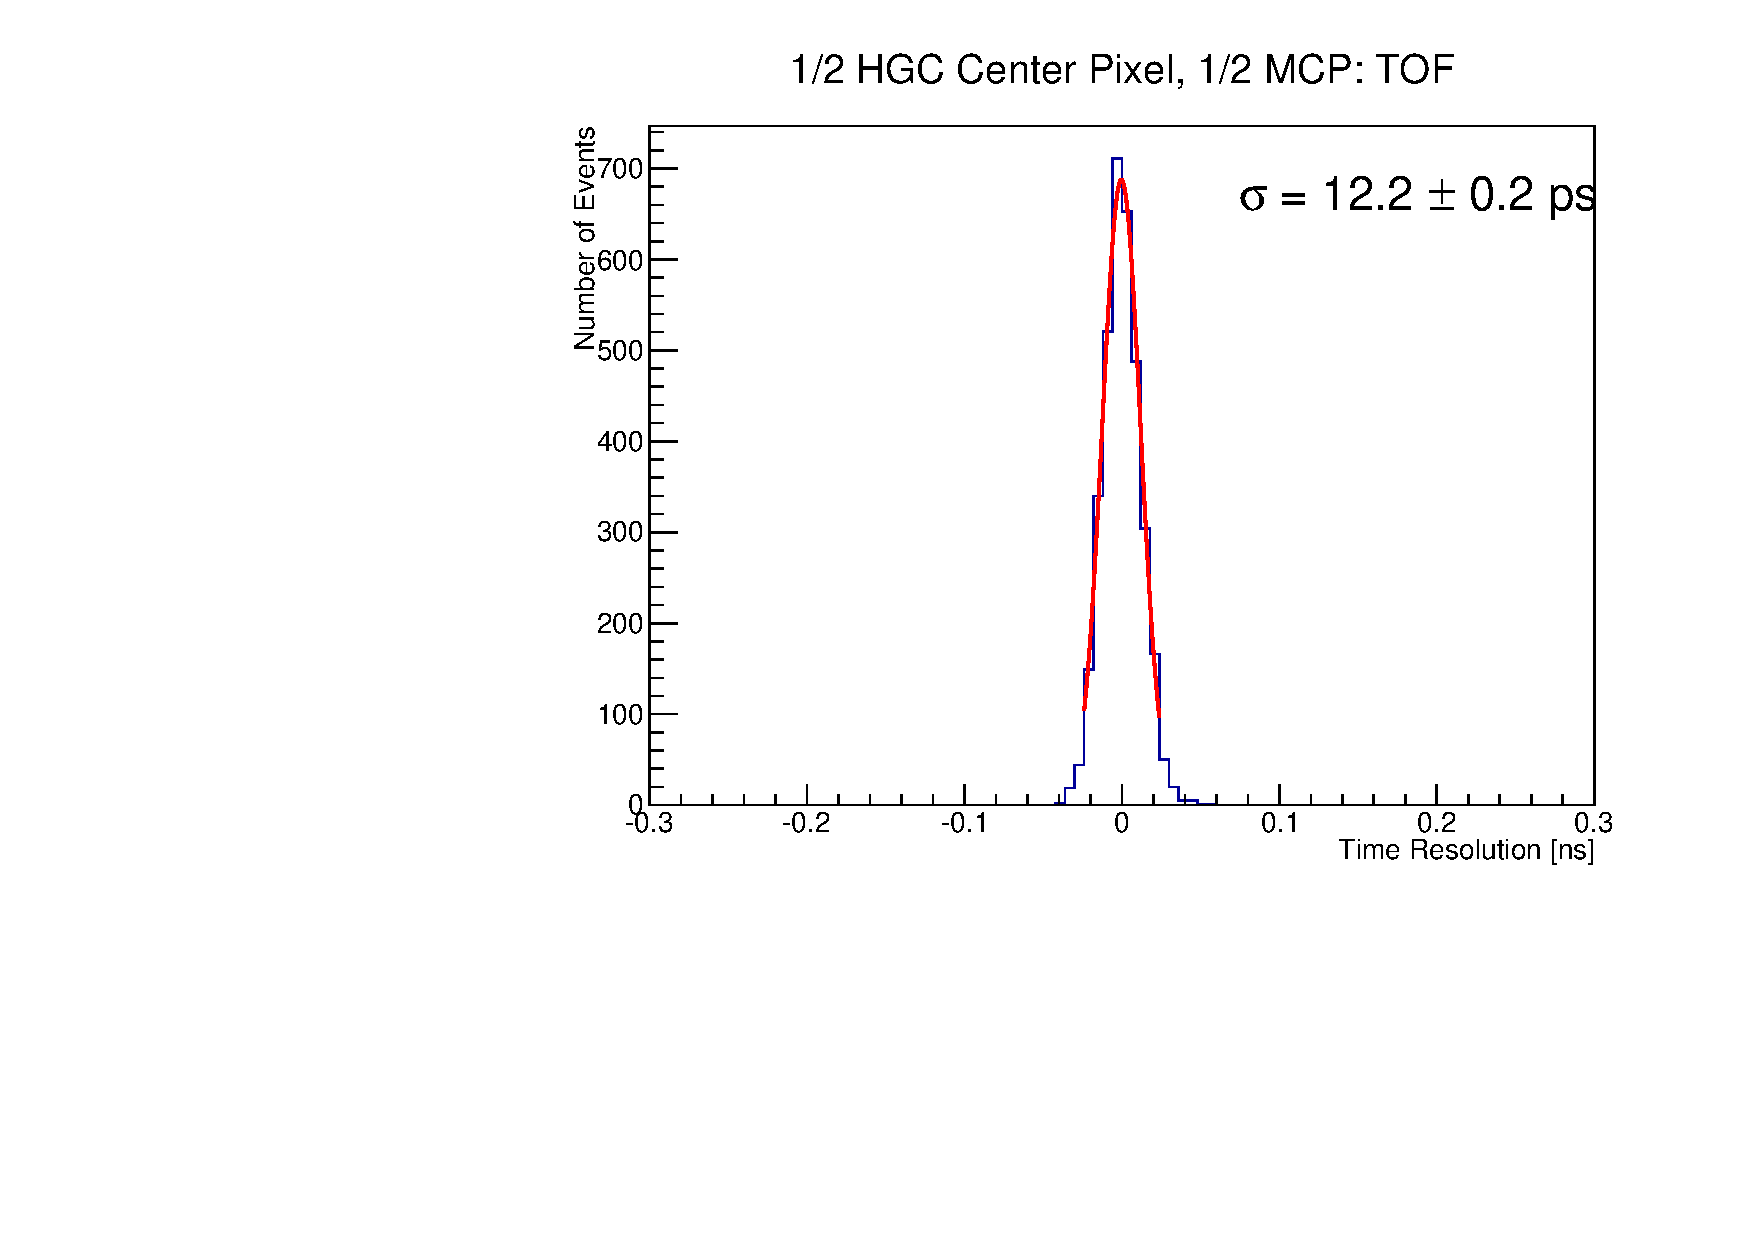
\includegraphics[width=\textwidth]{deltaT_Center_MCP_Equal.pdf}
	\caption{TOF histogram weighting $\Delta t_{Center}$ and $\Delta t_{Photonis}$ by $\frac{1}{2}$.}
	\label{fig:CenterMCPEqual}
\end{minipage} \hfill
\begin{minipage}[t]{.49\textwidth}
	\centering
	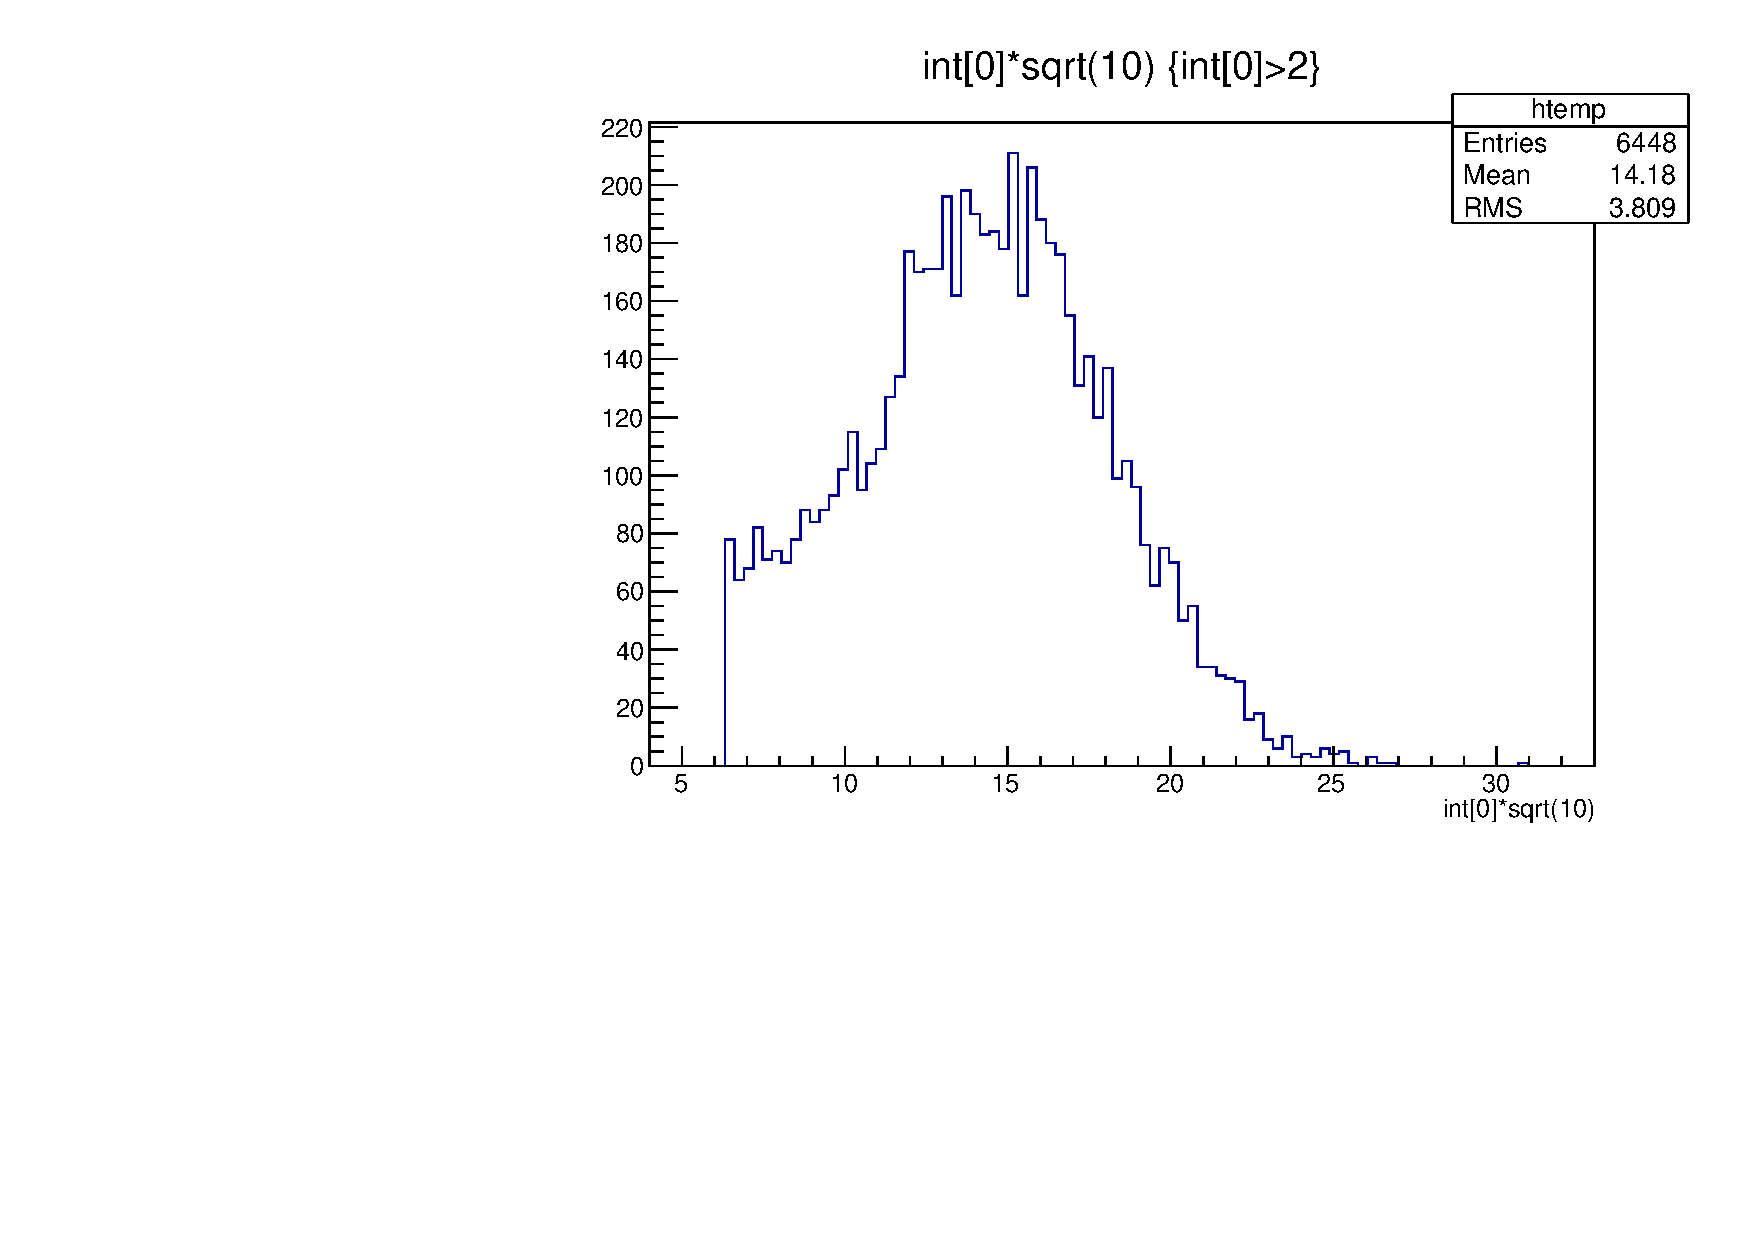
\includegraphics[width=\textwidth]{ChargeCut1.pdf}
	%\caption{The Photek 240 MCP charge distribution with the cut in effect. Zeroed charges represent events with only noise.}
	%\label{fig:ChargeCut1}
\end{minipage}
\end{figure}


\section{Preliminary Results}
I am currently using my analysis code for the HGC and MCP to look at how these time resolutions change for different configurations (i.e. absorber type, spacing, and thickness; beam energy; etc). 
So far, I have only looked at the following configurations:

%%% INCLUDE TABLE HERE %%%

The last run is a reminder that the cuts should be edited for every run in order to correctly select the proper data. 
There may also be a beam energy dependence for the value of the cuts. 
So far, I have determined that the following cuts are the best for the above runs:

%%% INCLUDE TABLE HERE %%%

As far as the rest of my research goes: I am going back to Caltech at the end of next week to continue my data analysis. 
I cannot really plan out how my analysis will evolve until I finish looking at the different runs, but then I will most likely take my results to someone in the Caltech Precision Timing group and figure out the next steps of my research. 

\begin{comment}
\begin{figure}
\centering
	\begin{minipage}[t]{.5\textwidth} % [t] aligns at top of minipage instead of centering it
	\centering
	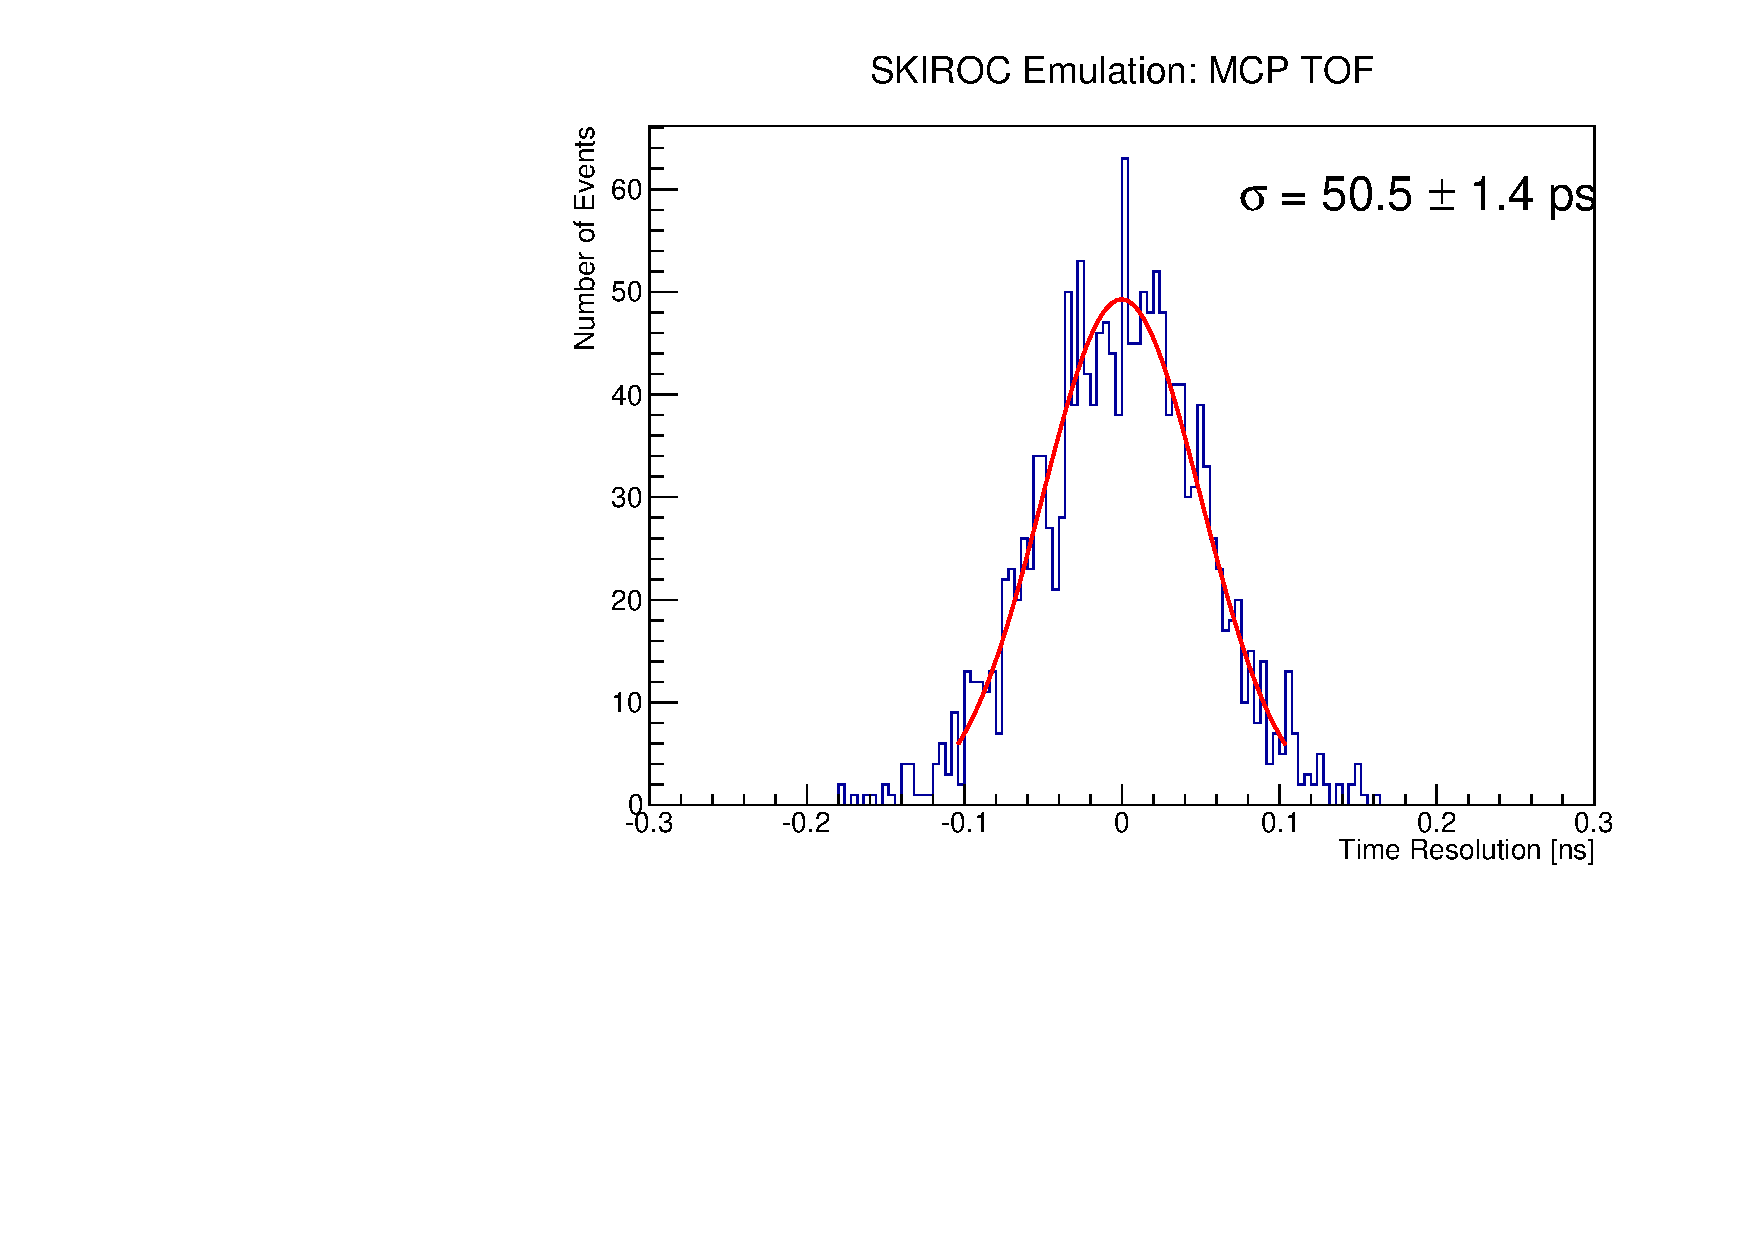
\includegraphics[width=\linewidth]{deltaTMCPSmear.pdf}
	\caption{Caption goes here}
	\label{peaks1}
	\end{minipage}\hfill
	\begin{minipage}[t]{.5\textwidth}
	\centering
	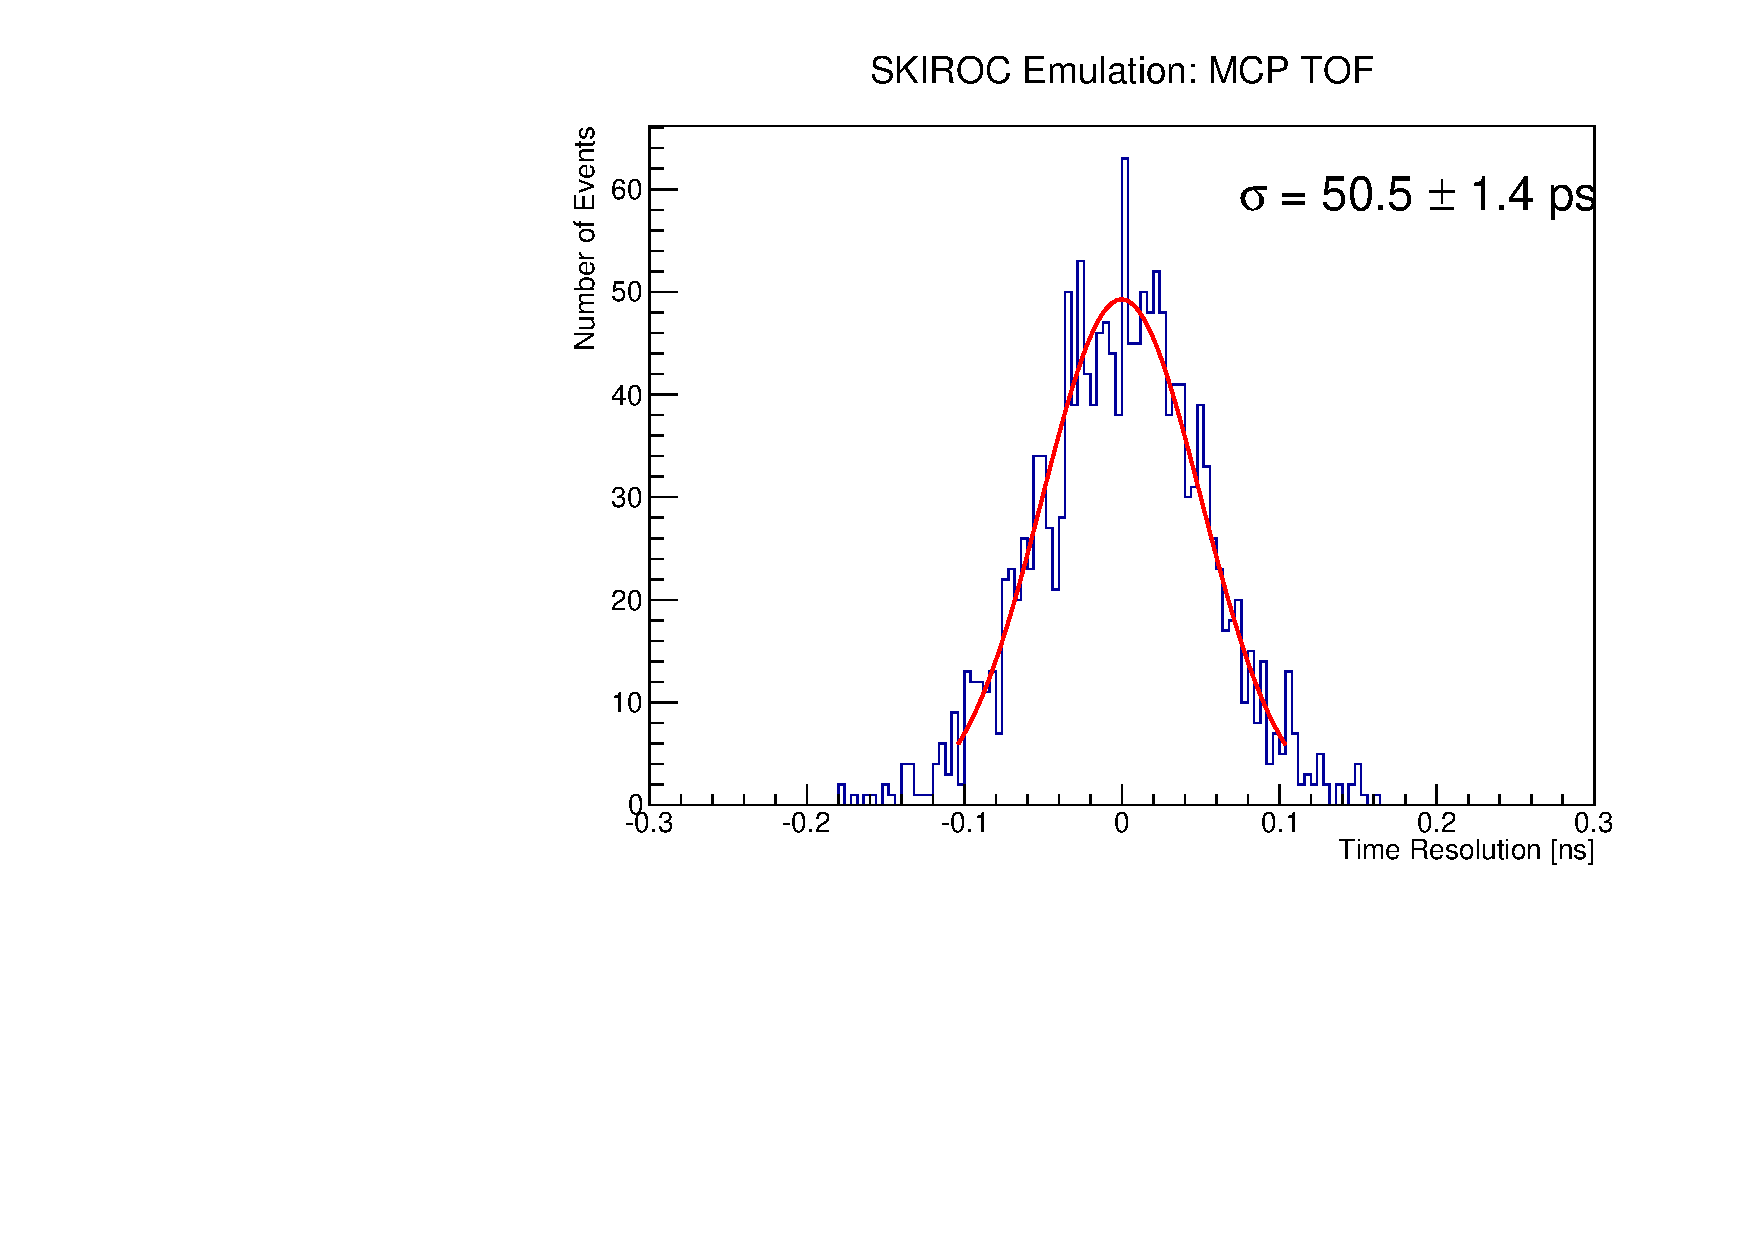
\includegraphics[width=\linewidth]{deltaTMCPSmear.pdf}
	\caption{Caption goes here}
	\label{peaks2}
	\end{minipage}
\end{figure}

look at \ref{peaks1} and \ref{peaks2}.
\end{comment}


\newpage
\printbibliography

\end{document}
